%!TeX spellcheck = pl_PL
\documentclass[11pt, a4paper, oneside]{report}
%jezyk dokumentu
\usepackage[utf8]{inputenc}
\usepackage[T1]{fontenc}
\usepackage[T1]{polski}
\usepackage[english, polish]{babel}
%\setlanguage{polish}
\usepackage{fullpage}
\usepackage{pdfpages}
%Style
\usepackage{siunitx,booktabs,threeparttable,caption}
\captionsetup[table]{justification=raggedright,singlelinecheck=off}
\sisetup{separate-uncertainty=true}
\raggedbottom

\captionsetup[figure]{justification=centering,singlelinecheck=off}
\sisetup{separate-uncertainty=true}

\setlength\parindent{0.5cm}
\renewcommand{\baselinestretch}{1.15} 
\makeatletter
\def\ps@myPS{%
    \def\@oddfoot{\null\hfill\thepage}
    \def\@evenfoot{\thepage}%
    \def\@evenhead{\null\hfil\slshape\leftmark}%
    \def\@oddhead{{\slshape\rightmark}}}%
\makeatother
\makeatletter
\renewcommand\chapter{
                    \thispagestyle{myPS}
                    \global\@topnum\z@
                    \@afterindentfalse
                    \secdef\@chapter\@schapter}
\makeatother
\makeatletter
\def\@makechapterhead#1{%
  \vspace*{50\p@}%
  {\parindent \z@ \raggedright \normalfont
    \interlinepenalty\@M
    \Huge\bfseries  \thechapter.\quad #1\par\nobreak
    \vskip 40\p@
  }}
\makeatother
\pagestyle{myPS}
%linkowanie
\usepackage{hyperref}
\hypersetup{
    colorlinks,
    citecolor=black,
    filecolor=black,
    linkcolor=black,
    urlcolor=black
}
\usepackage{multicol}
\usepackage{caption}
\usepackage{subcaption}
%math
\usepackage{amsmath}
\usepackage{gensymb}
\def\deg {$^o$\ }
\newcommand{\mat}[1]{\mathbf{#1}} % undergraduate algebra version
\newcommand{\sub}[1]{\footnotesize #1 \normalsize}
%bibliografia
\usepackage{csquotes}
\usepackage[backend=biber]{biblatex}
%,style=authoryear
%\renewcommand{\cite}[1]{\parencite{#1}}
\usepackage{float}
%numeracja
\usepackage{chngcntr}
%\counterwithout{figure}{chapter}	%numeracja ciagła
%oblsuga grafiki
\usepackage{graphicx}
\graphicspath{{../img/}{}../image/}
%time and date management
\usepackage{datetime}
\newcommand{\miesiac}{%
  \ifcase\THEMONTH
  \or Styczeń% 1
  \or Luty% 2
  \or Marzec% 3
  \or Kwiecień% 4
  \or Maj% 5
  \or Czerwiec% 6
  \or Lipiec% 7
  \or Sierpień% 8
  \or Wrzesień% 9
  \or Październik% 10
  \or Listopad% 11
  \or Grudzień% 12
  \fi}      
\newdateformat{mmyyyy}{\miesiac \  \THEYEAR}

%zarzadzanie tekstem
\brokenpenalty=1000		% nie dziel wyrazów miedzy stronami
\clubpenalty=1000		% kara za sierotki
\widowpenalty=10000		% nie pozostawiaj wdów

\usepackage[inner=30mm,outer=20mm,top=25mm,bottom=25mm]{geometry}

%Wyliczenia:
\usepackage{enumerate}

\usepackage{xr}
\usepackage{amsfonts}
\defbibheading{myheading}[Bibliografia]{%
  \chapter*{#1}
  \addcontentsline{toc}{chapter}{#1}}

\begin{document}

%Title page:


\begin{titlepage} 
	\newcommand{\HRule}{\rule{\linewidth}{0.5mm}}  
	\center 
	
	
\includegraphics[width = \textwidth]{logo.pdf} 
	\vfill 
	\textsc{\LARGE Projekt APSI}\\[1 cm] 

	\textsc{\large System informatyczny wspomagający zarządzanie pracownikami i projektami w firmie informatycznej}\\[0.5cm] 
	
	%------------------------------------------------
	%	Title
	%------------------------------------------------
	
	\HRule\\[0.4cm]
	
	{\huge\bfseries Moduł rejestru dostępnych zasobów}\\[0.4cm] 
	
	\HRule\\[1.5cm]
	
		\begin{center}
			\large
			\textsc{}{Zespół A06/17Z:}
            
			\textsc{Marcin Baran}
            
			\textsc{Hubert Grzegorz Buczyński}
            
			\textsc{Julia Czarnowska}
            
			\textsc{Maciej Krasowski}
		\end{center}
	
	\vfill\vfill\vfill 
	
	{\large 08.01.2018}
	
	
	\vfill % Push the date up 1/4 of the remaining page
	
\end{titlepage}

\counterwithin{subsection}{section}
\renewcommand{\thesubsection}{F%
\arabic{subsection}}
\tableofcontents
\pagebreak

\chapter{Wprowadzenie}

\section{Opis projektu}
Zadaniem systemu jest rejestracja i przechowywanie wszelkich dokumentów związanych z prowadzonymi projektami, jak również wspomaganie organizacji prac projektowych od specyfikowania wymagań aż do utrzymania systemu produkcyjnego. Celem implementacji naszego modułu jest dostarczenie możliwości zarządzaniem zasobami podczas realizacji projektów. 

\section{Procesy biznesowe}
W miarę rozrastania się przedsiębiorstwa a wraz z tym jego zasobów fizycznych procedury związane z zarządzaniem nimi stają coraz trudniejsze i mniej kontrolowalne. W związku z tym niezbędne jest narzędzie, które pozwoli na efektywne ewidencjonowanie różnego rodzaju zasobów dostępnych w przedsiębiorstwie.

\chapter{Słownik pojęć}
\begin{itemize}
\item system/moduł - moduł rejestru dostępnych zasobów,
\item zasób - każdy element dostępny w firmie wykorzystywany w pracy nad projektem. 
\item typ zasobu - zdefiniowana nazwa i zespół parametrów opisujący dany rodzaj zasobów

\end{itemize}

\chapter{Specyfikacja sprzętu i oprogramowania
podstawowego}
\paragraph{}
Wdrożenie aplikacji wymaga przygotowania odpowiedniego środowiska. Proponowana konfiguracja zakłada wykorzystanie serwera open-source Apache HTTP Server. Na serwerze przechowywane będą wszystkie dane systemu.

\paragraph{Środowisko sprzętowe}
\paragraph{}
Założenia odnośnie środowiska sprzętowego:
\begin{itemize}
\item Liczba osób aktywnie wykorzystujących aplikację mieści się w przedziale 50-100 użytkowników.
\item System jest użytkowany średnio 18 godzin na dobę.
\item Zasoby aplikacji są regularnie archiwizowane (transfer około 30GB miesięcznie)
\item System przechowuje zarchiwizowane zasoby (1 TB)
\end{itemize}

\paragraph{System operacyjny} 
\paragraph{} W projekcie wykorzystywane są narzędzia oraz technologie otwarte i ogólno dostępne, również system operacyjny. Sugerowanym systemem operacyjnym jest Linux.

\newpage


\chapter{Specyfikacja technologii}
\paragraph{} Aplikacja wykorzystuje szereg technologii, których połączenie pozwala uzyskać spójny i niezawodny system. Wśród zastosowanych technologii możemy wydzielić trzy zasadnicze podgrupy:

\begin{itemize}
\item technologie wykorzystywane przez serwer (back-end),
\item technologie użyte w interfejsie użytkownika (front-end),
\item technologie użyte do przechowywania danych.
\end{itemize}

\paragraph{Technologie użyte po stronie serwera}
	\paragraph{}
Głównym zadaniem serwera jest obsługa żądań napływających od użytkowników modułu przechwytywanych za pośrednictwem interfejsu użytkownika. Back-end aplikacji zostanie napisany w języku programowania Python. Język ten charakteryzuje sie szybką implementacją i dostępnością frameworków oraz bibliotek.

\paragraph{}
Do budowania i testowania kodu źródłowego zostanie zastosowana narzędzie Jenkins. W celu zapewnienia standaryzacji implementacja będzie opierać o szkielet tworzenia aplikacji Flask. Wykorzystane w aplikacji moduły frameworku:
\begin{itemize}
\item Login – używany do tworzenia sesji użytkownika,
\item SQLAlchemy - służący do obsługi bazy danych,
\item Migrate - tworzący back-up bazy danych,
\end{itemize}

\paragraph{Technologie wykorzystane do interfejsu użytkownika}
\paragraph{}
Interfejs użytkownika obsługiwany zostanie w aplikacji internetowej uruchomionej w przeglądarce, stworzonej w oparciu o framework AngularJS. Jest to jeden z najpopularniejszych szkieletów aplikacyjnych umożliwiający rozwój oprogramowania w stosunkowo krótkim czasie.

\paragraph{Technologie użyte do przechowywania danych}
\paragraph{}
Przechowywane przez system dane będą składowane w bazie danych MySQL. Ten system zarządzania bazą danych pozwala na zdefiniowanie różnych użytkowników oraz nadanie im różnych praw dostępu. Ta funkcjonalność pozwala na zabezpieczenie przed nieautoryzowanym dostępem do przechowywanych danych przez osoby niepożądane. Ponadto jest to rozwiązanie opensource.
\newpage


\chapter{Aktorzy}
Ze względu na przysługujące uprawnienia oraz spełniane funkcje w systemie zidentyfikowano następujących aktorów:
\begin{itemize}
\item użytkownik – podstawowy aktor posiadający ograniczone prawa do systemu, wynikające z pełnionej przez niego funkcji w firmie,
\item administrator systemu – osoba odpowiedzialna za zarządzanie oraz administrowanie pracą systemu, 
\item użytkownik techniczny - użytkownik odpowiedzialny za rejestrację oraz stan techniczny przynależnych mu zasobów, 
\item menedżer - osoba decyzyjna, weryfikująca zgłoszenia o zasoby, mająca możliwość jego zatwierdzenia bądź odrzucenia.
\end{itemize}
\begin{figure}[H]
Diagram podziału użytkowników:

\centering
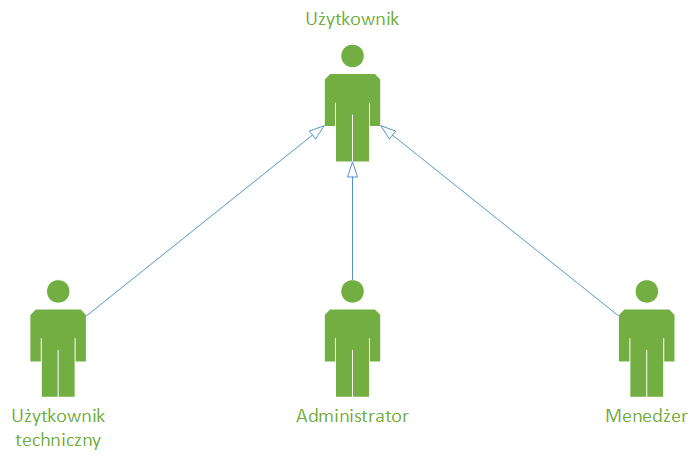
\includegraphics[scale=1]{Dziedziczenie.png}
\end{figure}

\chapter{Wymagania funkcjonalne}
\counterwithout{subsection}{section}
\counterwithin{subsection}{chapter}
\renewcommand{\thesubsection}{\colorbox{green}{\textcolor{white}{F%
\arabic{subsection}}}}
\section{Weryfikacja użytkowników}
\subsection{Użytkownik może zalogować się na swoje konto.}
\begin{center}
\begin{tabular}[c]{| l | l | }
  \hline			
  Priorytet realizacji & 10 \\
  \hline
  Złożoność realizacji & 5 \\
  \hline  
\end{tabular}
\end{center}
\subsection{Użytkownik może wylogować się w każdej chwili pracy w module.}
\begin{center}
\begin{tabular}[c]{| l | l | }
  \hline			
  Priorytet realizacji & 10 \\
  \hline
  Złożoność realizacji & 4 \\
  \hline  
\end{tabular}
\end{center}
\subsection{Użytkownicy mają zdefiniowane prawa dostępu.}
\begin{center}
\begin{tabular}[c]{| l | l | }
  \hline			
  Priorytet realizacji & 8 \\
  \hline
  Złożoność realizacji & 6 \\
  \hline  
\end{tabular}
\end{center}
\subsection{W zależności od nadanych praw użytkownicy mają różny zakres funkcjonalności modułu.}
\begin{center}
\begin{tabular}[c]{| l | l | }
  \hline			
  Priorytet realizacji & 8 \\
  \hline
  Złożoność realizacji & 7 \\
  \hline  
\end{tabular}
\end{center}

\subsection{W przypadku trzykrotnego niepowodzenia przy logowaniu konto użytkownika zostaje zablokowane na czas jednej godziny.}
\begin{center}
\begin{tabular}[c]{| l | l | }
  \hline			
  Priorytet realizacji & 7 \\
  \hline
  Złożoność realizacji & 4 \\
  \hline  
\end{tabular}
\end{center}
\subsection{W sytuacji, gdy sesja użytkownika jest nieaktywna dłużej niż piętnaście minut, użytkownik zostaje automatycznie wylogowany.}
\begin{center}
\begin{tabular}[c]{| l | l | }
  \hline			
  Priorytet realizacji & 6 \\
  \hline
  Złożoność realizacji & 5 \\
  \hline  
\end{tabular}
\end{center}

\section{Konta użytkowników:}
\subsection{Użytkownik z prawami dostępu administratora ma możliwość stworzenia i zatwierdzenia konta użytkownika ubiegającego się o nie.}
\begin{center}
\begin{tabular}[c]{| l | l | }
  \hline			
  Priorytet realizacji & 10 \\
  \hline
  Złożoność realizacji & 5 \\
  \hline  
\end{tabular}
\end{center}
\subsection{Użytkownik z prawami dostępu administratora ma możliwość usuwania kont użytkowników modułu.}
\begin{center}
\begin{tabular}[c]{| l | l | }
  \hline			
  Priorytet realizacji & 9 \\
  \hline
  Złożoność realizacji & 6 \\
  \hline  
\end{tabular}
\end{center}
\subsection{Użytkownik z prawami dostępu administratora ma możliwość edycji praw dostępu istniejących użytkowników w module.}
\begin{center}
\begin{tabular}[c]{| l | l | }
  \hline			
  Priorytet realizacji & 10 \\
  \hline
  Złożoność realizacji & 5 \\
  \hline  
\end{tabular}
\end{center}

\subsection{Użytkownik z prawami dostępu administratora ma możliwość podglądu historii zasobu.}
\begin{center}
\begin{tabular}[c]{| l | l | }
  \hline			
  Priorytet realizacji & 10 \\
  \hline
  Złożoność realizacji & 7 \\
  \hline  
\end{tabular}
\end{center}
\subsection{Użytkownik z prawami dostępu administratora ma możliwość podglądu historii użytkownika.}
\begin{center}
\begin{tabular}[c]{| l | l | }
  \hline			
  Priorytet realizacji & 8 \\
  \hline
  Złożoność realizacji & 7 \\
  \hline  
\end{tabular}
\end{center}
\section{Zarządzanie zasobami:}
\subsection{Użytkownik techniczny ma możliwość dodawania nowych i usuwania istniejących zasobów przynależnych do danego typu.}
\begin{center}
\begin{tabular}[c]{| l | l | }
  \hline			
  Priorytet realizacji & 10 \\
  \hline
  Złożoność realizacji & 8 \\
  \hline  
\end{tabular}
\end{center}
\subsection{Użytkownik techniczny ma możliwość, po uprzednim  stwierdzeniu przez menedżera, przyznawania zasobów użytkownikom, którzy złożyli na nie zamówienie.}
\begin{center}
\begin{tabular}[c]{| l | l | }
  \hline			
  Priorytet realizacji & 10 \\
  \hline
  Złożoność realizacji & 8 \\
  \hline  
\end{tabular}
\end{center}
\subsection{Użytkownik techniczny ma możliwość modyfikacji danych zasobu.}
\begin{center}
\begin{tabular}[c]{| l | l | }
  \hline			
  Priorytet realizacji & 10 \\
  \hline
  Złożoność realizacji & 6 \\
  \hline  
\end{tabular}
\end{center}
\subsection{Użytkownik techniczny ma możliwość wprowadzania historii napraw zasobów dokonywanych w firmie jak i przez serwis zewnętrzny.}
\begin{center}
\begin{tabular}[c]{| l | l | }
  \hline			
  Priorytet realizacji & 9 \\
  \hline
  Złożoność realizacji & 6 \\
  \hline  
\end{tabular}
\end{center}
\subsection{Wszelkie modyfikacje zasobu zapisywane są w jego historii. }
\begin{center}
\begin{tabular}[c]{| l | l | }
  \hline			
  Priorytet realizacji & 9 \\
  \hline
  Złożoność realizacji & 5 \\
  \hline  
\end{tabular}
\end{center}
\subsection{Każdy użytkownik ma możliwość podglądu przypisanych do niego w danej chwili zasobów.}
\begin{center}
\begin{tabular}[c]{| l | l | }
  \hline			
  Priorytet realizacji & 10 \\
  \hline
  Złożoność realizacji & 6 \\
  \hline  
\end{tabular}
\end{center}
\subsection{Użytkownik techniczny ma możliwość podglądu wszystkich zasobów, za które jest odpowiedzialny.}
\begin{center}
\begin{tabular}[c]{| l | l | }
  \hline			
  Priorytet realizacji & 10 \\
  \hline
  Złożoność realizacji & 7 \\
  \hline  
\end{tabular}
\end{center}
\subsection{Użytkownik techniczny/Administrator ma możliwość przeglądania wszystkich zasobów według zdefiniowanych przez siebie kryteriów (np. posortowane, zgodne z wybranymi filtrami).}
\begin{center}
\begin{tabular}[c]{| l | l | }
  \hline			
  Priorytet realizacji & 8 \\
  \hline
  Złożoność realizacji & 7 \\
  \hline  
\end{tabular}
\end{center}
\subsection{Administrator ma możliwość przeglądania wszystkich zasobów według zdefiniowanych przez siebie kryteriów (np. posortowane, zgodne z wybranymi filtrami).}
\begin{center}
\begin{tabular}[c]{| l | l | }
  \hline			
  Priorytet realizacji & 8 \\
  \hline
  Złożoność realizacji & 7 \\
  \hline  
\end{tabular}
\end{center}

\subsection{Użytkownik ma możliwość zgłoszenia chęci skorzystania z zasobu.}
\begin{center}
\begin{tabular}[c]{| l | l | }
  \hline			
  Priorytet realizacji & 9 \\
  \hline
  Złożoność realizacji & 7 \\
  \hline  
\end{tabular}
\end{center}
\subsection{Użytkownik ma możliwość zgłoszenia zasobu do serwisu.}
\begin{center}
\begin{tabular}[c]{| l | l | }
  \hline			
  Priorytet realizacji & 9 \\
  \hline
  Złożoność realizacji & 7 \\
  \hline  
\end{tabular}
\end{center}
\subsection{Użytkownik technicznych ma możliwość zmiany statusu zasobu na serwisowany.}
\begin{center}
\begin{tabular}[c]{| l | l | }
  \hline			
  Priorytet realizacji & 9 \\
  \hline
  Złożoność realizacji & 8 \\
  \hline  
\end{tabular}
\end{center}

\section{Zarządzanie typami zasobów:}
\subsection{Administrator ma możliwość dodawania i usuwania typów zasobów}
\begin{center}
\begin{tabular}[c]{| l | l | }
  \hline			
  Priorytet realizacji & 10 \\
  \hline
  Złożoność realizacji & 8 \\
  \hline  
\end{tabular}
\end{center}

\subsection{Administrator ma możliwość edycji zespołu parametrów istniejących typów zasobów.}
\begin{center}
\begin{tabular}[c]{| l | l | }
  \hline			
  Priorytet realizacji & 10 \\
  \hline
  Złożoność realizacji & 8 \\
  \hline  
\end{tabular}
\end{center}

\section{Zarządzanie modułem:}
\subsection{Administrator ma możliwość przywracania ustawień fabrycznych modułu.}
\begin{center}
\begin{tabular}[c]{| l | l | }
  \hline			
  Priorytet realizacji & 9 \\
  \hline
  Złożoność realizacji & 5 \\
  \hline  
\end{tabular}
\end{center}

\subsection{Administrator ma możliwość tworzenia kopii zapasowej danych.}
\begin{center}
\begin{tabular}[c]{| l | l | }
  \hline			
  Priorytet realizacji & 9 \\
  \hline
  Złożoność realizacji & 6 \\
  \hline  
\end{tabular}
\end{center}

\subsection{Administrator ma możliwość tworzenia kopii zapasowej danych.}
\begin{center}
\begin{tabular}[c]{| l | l | }
  \hline			
  Priorytet realizacji & 9 \\
  \hline
  Złożoność realizacji & 6 \\
  \hline  
\end{tabular}
\end{center}

\section{Generowanie raportów:}
\subsection{Użytkownik techniczny/Administrator ma możliwość, po uprzednim określeniu kryteriów, wygenerowania raportu w postaci pliku pdf.}
\begin{center}
\begin{tabular}[c]{| l | l | }
  \hline			
  Priorytet realizacji & 7 \\
  \hline
  Złożoność realizacji & 7 \\
  \hline  
\end{tabular}
\end{center}

\chapter{Wymagania niefunkcjonalne}
\counterwithout{subsection}{section}
\counterwithin{subsection}{chapter}
\renewcommand{\thesubsection}{\colorbox{blue}{\textcolor{white}{NF%
\arabic{subsection}}}}
\section{Ergonomia:}
\subsection{Interfejs}
System powinien posiadać intuicyjny interfejs użytkownika.
\subsection{Przenośność systemu}
Dostęp do systemu powinien być zapewniony z poziomu różnych platform w tym platform mobilnych, dlatego interfejs aplikacji powinien wspierać także te rozwiązania.
\subsection{Język systemu}
System powinien posiadać interfejs w języku polskim oraz angielskim.
\section{Dostępność systemu:}
\subsection{Okres dostępności}
System powinien być dostępny 99.999\% czasu.
\subsection{Czas naprawy}
System powinien zostać skonstruowany, w taki sposób, aby naprawa przebiegała w możliwie najkrótszym czasie.
\subsection{Kompatybilność}
System powinien być kompatybilny z systemami Windows (od wersji 7) oraz Linux.
\subsection{Awaria systemu}
Czas awarii systemu nie powinien być dłuższy niż 1 godzina.
\subsection{Dostęp do systemu}
Dostęp do systemu powinien być zapewniony poprzez stronę internetową.
\section{Wydajność:}
\subsection{Czas zapytania} 
System powinien zapewniać możliwość wykonania prośby o przyznanie konkretnego zasobu w czasie poniżej 3 sekund.
\subsection{Eksport danych}
System powinien zapewniać możliwość eksportowania danych do pliku o wielkości nie większej niż 10 MB w czasie nie większym niż 10 sekund.
\section{Bezpieczeństwo i utrzymanie:}
\subsection{Serwisowanie systemu}
Prace związane z naprawą i serwisowaniem powinny być wykonywane możliwie w czasie późnych godzin (prawdopodobnie o 03:30 czasu lokalnego).
\subsection{Aktualizacje}
Aktualizacje powinny być wykonywane zgodnie z harmonogramem określonym w punkcie 6.4.1.
\subsection{Komunikacja z serwerem}
Komunikacja pomiędzy serwerem i klientem powinna przebiegać przez łącze VPN.
\subsection{Integralność danych}
System powinien posiadać weryfikację wprowadzanych danych.
\subsection{Backup bazy danych}
System powinien robić backup bazy danych codziennie podczas małego obciążenia (prawdopodobnie o 03:30 w nocy). Nie powinno to się dziać kosztem dostępności.
\subsection{Zabezpieczenie połączenia}
Połączenie z serwerem jest szyfrowane.
\subsection{Logi systemu}
System powinien generować logi zawierające informacje o zmianach dokonywanych przez użytkowników oraz informacje diagnostyczne.
\subsection{Nieautoryzowany dostęp}
System powinien wykrywać próby nieautoryzowanego dostępu i informować o nich administratora.

\subsection{Błędne logowanie}
System powinien blokować możliwość logowania dla adresu IP, z którego zostały wykonane 3 nieudane próby logowania.
\section{Projektowanie}
\subsection{Technologia wykonania}
System powinien być wykonany przy użyciu technologii, które są spójne z polityką i kierunkiem rozwoju firmy.

\subsection{Rozszerzanie funkcjonalności}
System powinien zapewniać możliwość elastycznego rozszerzania funkcjonalności.

\section{Skalowalność}
\subsection{Rozrastanie się systemu}
System powinien mieć możliwość rozrastania się w miarę rozwoju bazy zasobów bez konieczności modyfikacji oprogramowania.

\chapter{Przypadki użycia}
\counterwithin{subsection}{section}
\renewcommand{\thesection}{\colorbox{red}{\textcolor{white}{PU%
\arabic{section}}}}

\section{Logowanie użytkownika}
\paragraph{Opis przypadku użycia:}
Użytkownik może się zalogować do modułu zarządzania zasobami firmy.
\paragraph{Priorytet:} 10
\paragraph{Aktorzy:} Użytkownik
\paragraph{Podstawowy przebieg:}
Ten przypadek użycia zaczyna się gdy użytkownik wchodzi na stronę logowania do modułu.
Użytkownik podaje dane do logowania i system sprawdza ich poprawność
Użytkownik ma możliwość zresetowania hasła, które zostanie przesłane na podany przez niego e-mail, jeśli ten znajduje się w bazie użytkowników.
\paragraph{Przebiegi alternatywne:} 
PU1.A Nieprawidłowa nazwa użytkownika/hasła:
Jeśli użytkownik podał złą nazwę użytkownika lub hasło system wyświetla odpowiedni komunikat błędu. Aktor w tym momencie może zdecydować by wrócić do początku przebiegu podstawowego lub anulować logowanie, co kończy ten przypadek użycia.

PU1.B Czasowe zablokowanie konta:
Jeżeli użytkownik w ciągu 10 minut trzykrotnie wykona nieudane próby logowania system zablokuje mu możliwość kolejnej próby na 1 godzinę


\begin{figure}[H]
Diagram przypadku użycia:

\centering
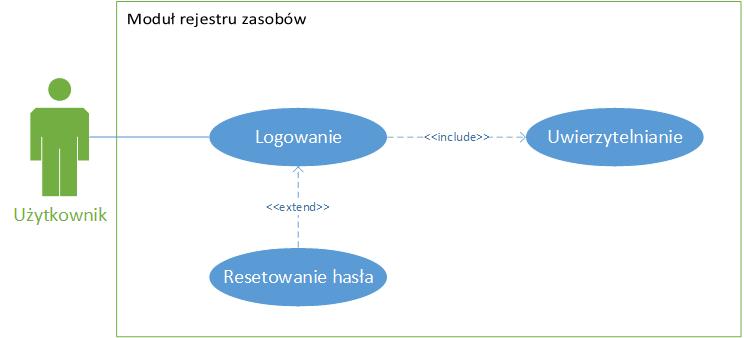
\includegraphics[scale=1]{uzytkownik_logowanie.png}
\end{figure}

\paragraph{Warunki wstępne:} Użytkownik jest zarejestrowany w module.
\paragraph{Warunki końcowe:} Jeśli przypadek użycia został poprawnie zrealizowany to aktor jest zalogowany do modułu.

\section{Rejestracja użytkownika}
\paragraph{Opis przypadku użycia:} Administrator ma możliwość stworzenia konta dla nowego użytkownika.
\paragraph{Priorytet:} 10
\paragraph{Aktorzy:} Administrator
\paragraph{Podstawowy przebieg:}
W tym przypadku użycia administrator tworzy nowe konto dla użytkownika definiując w nim prawa dostępu oraz login i hasło niezbędne w procesie logowania.
System potwierdza poprawność danych.
Administrator zatwierdza konto użytkownika.

\paragraph{Przebiegi alternatywne:}

PU2.A Nieprawidłowa nazwa użytkownika

Jeśli administrator podał nazwę użytkownika, która jest już używana w systemie lub hasło, które nie spełnia wymogów systemowych, system wyświetla odpowiedni komunikat błędu. Aktor w tym momencie może zdecydować by wrócić do początku przebiegu podstawowego lub anulować rejestrację, co kończy ten przypadek użycia.

\begin{figure}[H]
Diagram przypadku użycia:

\centering
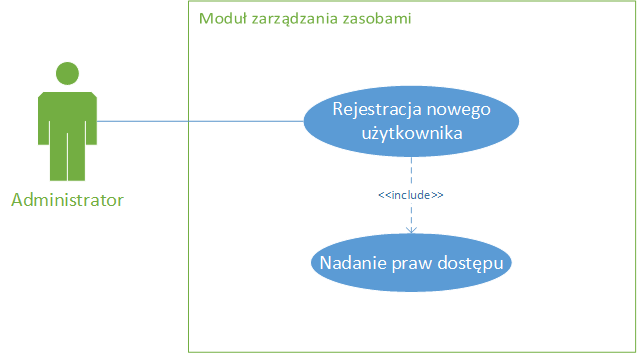
\includegraphics[scale=1]{uzytkownik_rejestracja.png}
\end{figure}
\paragraph{Warunki wstępne:} Administrator musi być zalogowany.
\paragraph{Warunki końcowe:}
Użytkownik ma funkcjonujące konto z należnymi dla swojej funkcji prawami użytkownika.
\section{Zgłoszenie o przyznanie nowego zasobu} 
\paragraph{Opis przypadku użycia:}
Użytkownik ma możliwość wprowadzenia do systemu zgłoszenia o nowy zasób.
\paragraph{Priorytet:} 9
\paragraph{Aktorzy:} Użytkownik
\paragraph{Podstawowy przebieg:}
Użytkownik zgłasza prośbę o przyznanie zasobu o wybranym typie. 

\begin{figure}[H]
Diagram przypadku użycia:

\centering
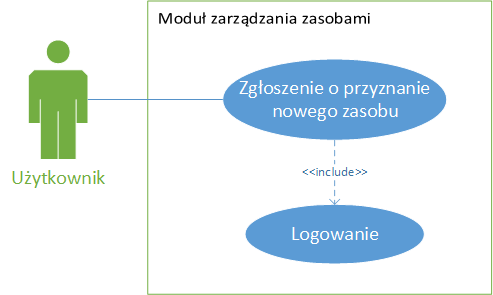
\includegraphics[scale=1]{uzytkownik_zgloszenie_o_zasob.png}
\end{figure}

\paragraph{Warunki wstępne:} Użytkownik musi być zalogowany.
\paragraph{Warunki końcowe:} Zgłoszenie zostaje przekazane do użytkownika technicznego.

\section{Zatwierdzenie zgłoszenia o zasób dla użytkownika}
\paragraph{Opis przypadku użycia:} Menedżer ma możliwość zatwierdzenia zgłoszenia o nowy zasób, które wystawił użytkownik.
\paragraph{Priorytet:} 7
\paragraph{Aktorzy:} Menedżer
\paragraph{Podstawowy przebieg:}
Menedżer zatwierdza zgłoszenie o nowy zasób.

\paragraph{Przebieg alternatywny:}
PU4.A Menedżer odrzuca zgłoszenie: Jeżeli menedżer odrzuci zgłoszenie, użytkownik zostaje o nim powiadomiony i może wystawić nowy, poprawiony wniosek.

\begin{figure}[H]
Diagram przypadku użycia:

\centering
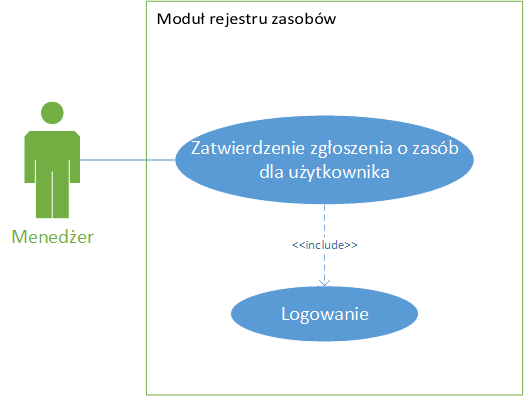
\includegraphics[scale=1]{menedzer_zasoby.png}
\end{figure}

\paragraph{Warunki wstępne:} Menedżer musi być zalogowany.
\paragraph{Warunki końcowe:} Menedżer zatwierdza zgłoszenie i jest ono przekazane do działu technicznego.

\section{Wydanie zasobu}
\paragraph{Opis przypadku użycia:} 
Użytkownik techniczny ma możliwość przekazania zasobu dla użytkownika, który zgłosił o niego zapotrzebowanie.
\paragraph{Priorytet:} 8
\paragraph{Aktorzy:} Użytkownik techniczny
\paragraph{Podstawowy przebieg:}
\begin{enumerate}
\item Użytkownik techniczny przyjmuje zatwierdzone zgłoszenie od menedżera.
\item Użytkownik techniczny przypisuje zasób do konta użytkownika.
\end{enumerate}

\begin{figure}[H]
Diagram przypadku użycia:

\centering
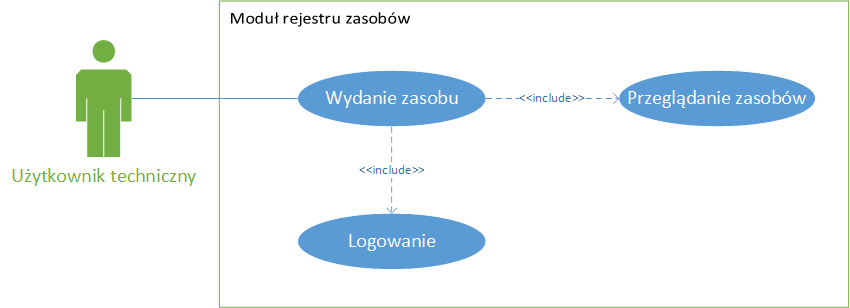
\includegraphics[scale=0.8]{wydanie_zasobu.png}
\end{figure}

\paragraph{Warunki wstępne:} Użytkownik techniczny musi być zalogowany. Menedżer musi zatwierdzić zgłoszenie.
\paragraph{Warunki końcowe:} Użytkownik techniczny przepisuje zasób na użytkownika zgłaszającego zapotrzebowanie.

\section{Zgłoszenie zasobu do serwisu}
\paragraph{Opis przypadku użycia:}
Użytkownik ma możliwość zgłoszenia wadliwego/zniszczonego zasobu do serwisu w celu naprawy.
\paragraph{Priorytet:} 5
\paragraph{Aktorzy:} Użytkownik
\paragraph{Podstawowy przebieg:}
Użytkownik zgłasza zasób, który uległ awarii do serwisu.
\paragraph{Przebiegi alternatywne:}
PU6.A Użytkownik omyłkowo zgłosił zasób do serwisu.
\newline Jeśli użytkownik zgłosił zły zasób, może to cofnąć jednym przyciskiem.
\begin{figure}[H]
Diagram przypadku użycia:

\centering
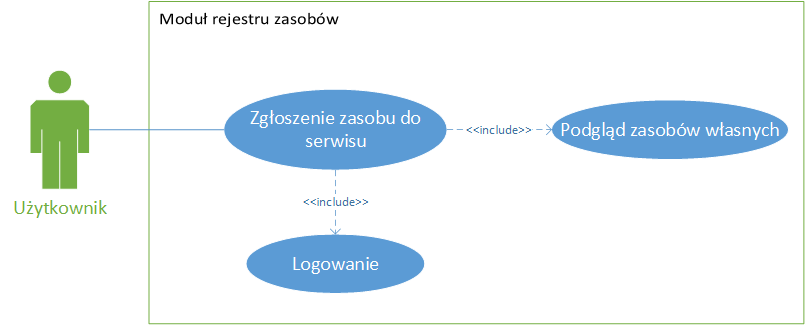
\includegraphics[scale=0.8]{uzytkownik_zgloszenie_do_serwisu.png}
\end{figure}

\paragraph{Warunki wstępne:} Użytkownicy muszą być zalogowani.
\paragraph{Warunki końcowe:} Zgłoszenie zostaje przekazane do serwisu.


\section{Przyjęcie zgłoszenia serwisowego}
\paragraph{Opis przypadku użycia:} Użytkownik techniczny ma możliwość przyjęcia zgłoszenia do serwisu wadliwego zasobu.
\paragraph{Priorytet:} 10
\paragraph{Aktorzy:} Użytkownik techniczny
\paragraph{Podstawowy przebieg:}
Użytkownik techniczny przyjmuje nowe zgłoszenie serwisowe od użytkownika i zapisuje je do serwisu wewnętrznego.
\paragraph{Przebieg alternatywny:}
PU7.A Usunięcie wadliwego zasobu:
W przypadku usterki niemożliwej do naprawy, użytkownik techniczny oznacza zasób jako usunięty.

PU7.B Zgłoszenie do serwisu zewnętrznego:
W sytuacji gdy zasób wymaga naprawy przez serwis zewnętrzny, użytkownik techniczny odnotowuje w systemie serwis, do którego zasób został przesłany.
\begin{figure}[H]
Diagram przypadku użycia:

\centering
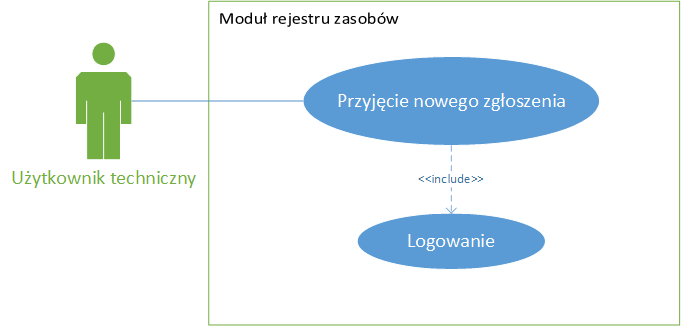
\includegraphics[scale=1]{uzytkownik_tech_serwis.png}
\end{figure}

\paragraph{Warunki wstępne:} Użytkownik musi być zalogowany.
\paragraph{Warunki końcowe:} Zgłoszenie zostaje zamknięte, a historia naprawy jest zapisana w systemie.

\section{Wylogowanie}
\paragraph{Opis przypadku użycia:} Użytkownik ma możliwość wylogowania się z systemu.
\paragraph{Priorytet:} 10
\paragraph{Aktorzy:} Użytkownik
\paragraph{Podstawowy przebieg:}
Użytkownik zaznacza w systemie jednym przyciskiem, że chce się wylogować z modułu i zakończyć sesję.

\begin{figure}[H]
Diagram przypadku użycia:

\centering
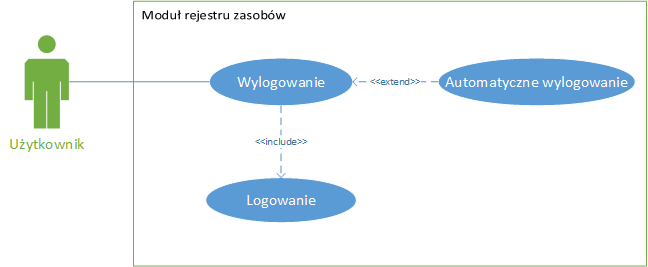
\includegraphics[scale=1]{uzytkownik_wylog.png}
\end{figure}

\paragraph{Warunki wstępne:} Użytkownik musi być zalogowany.
\paragraph{Warunki końcowe:} Użytkownik jest wylogowany i musi się ponownie zalogować w celu korzystania z modułu.

\section{Zgłoszenie o kupno zasobu}
\paragraph{Opis przypadku użycia:} Menedżer ma możliwość złożyć zgłoszenie o kupno nowego zasobu wymaganego w projekcie. 
\paragraph{Priorytet:} 4
\paragraph{Aktorzy:} Menedżer
\paragraph{Podstawowy przebieg:}
Menedżer składa zapotrzebowanie na nowy zasób, który nie znajduje się w systemie.
\paragraph{Przebiegi alternatywne:}

--

\begin{figure}[H]
Diagram przypadku użycia:

\centering
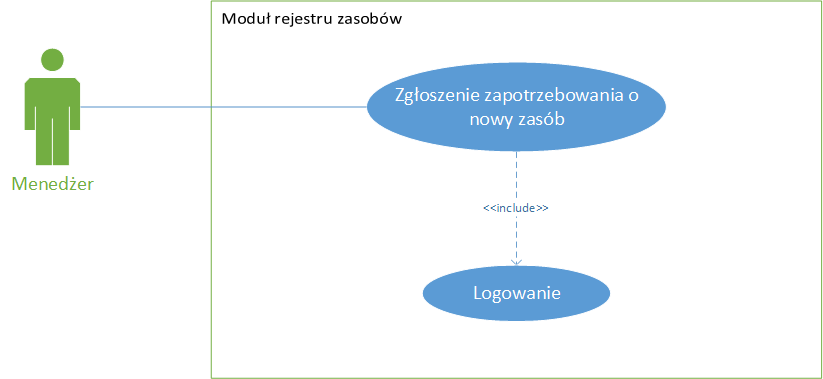
\includegraphics[scale=0.8]{nowy_zasob_menedzer_techniczny.png}
\end{figure}

\paragraph{Warunki wstępne:} Menedżer musi być zalogowany.
\paragraph{Warunki końcowe:} Zgłoszenie zostaje przekazane do realizacji.

\section{Kupno zasobu}
\paragraph{Opis przypadku użycia:} Użytkownik techniczny ma możliwość zakupienia nowego zasobu.
\paragraph{Priorytet:} 4
\paragraph{Aktorzy:} Użytkownik techniczny
\paragraph{Podstawowy przebieg:}
Użytkownik techniczny dokonuje zakupu zasobu.
\paragraph{Przebiegi alternatywne:}

PU10.A Użytkownik techniczny nie mógł zrealizować zamówienia.

Jeśli użytkownik techniczny z różnych powodów nie był w stanie zrealizować zamówienie takie wydarzenie zostaje odnotowane w systemie i odpowiednia informacja dociera do menadżera składającego zapotrzebowanie.

\begin{figure}[H]
Diagram przypadku użycia:

\centering
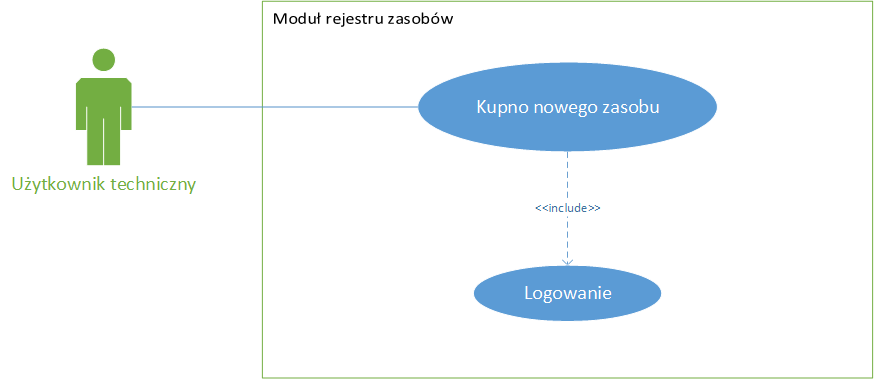
\includegraphics[scale=0.8]{techniczny_kupno.png}
\end{figure}

\paragraph{Warunki wstępne:} Menedżer musi zgłosić zapotrzebowanie na nowy zasób.
\paragraph{Warunki końcowe:} Użytkownik techniczny zamyka zgłoszenie kupna zasobu.

\section{Podgląd historii użytkowników}
\paragraph{Opis przypadku użycia:} Administrator może weryfikować poczynania wybranego użytkownika systemu.
\paragraph{Priorytet:} 8
\paragraph{Aktorzy:} Administrator
\paragraph{Podstawowy przebieg:}
\begin{enumerate}
\item Administrator może sprawdzać historię operacji użytkownika w systemie.
\end{enumerate}

\begin{figure}[H]
Diagram przypadku użycia:

\centering
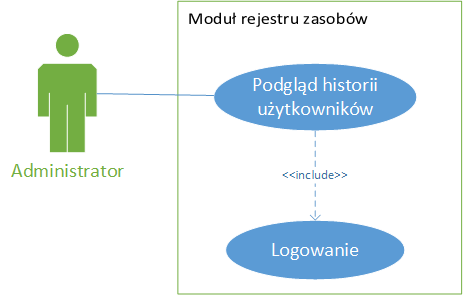
\includegraphics[scale=1]{admin_statystyki.png}
\end{figure}

\paragraph{Warunki wstępne:} Administrator musi być zalogowany.
\paragraph{Warunki końcowe:} ---

\section{Zarządzanie modułem}
\paragraph{Opis przypadku użycia:} Administrator ma możliwość zarządzania modułem systemu odpowiadającego za gospodarowanie zasobami przedsiębiorstwa.
\paragraph{Priorytet:} 9
\paragraph{Aktorzy:} Administrator
\paragraph{Podstawowy przebieg:}
\begin{enumerate}
\item Administrator ma możliwość zarządzania kontem wybranego użytkownika
\item Administrator ma możliwosć weryfikacji stanu zasobów
\item Administrator ma możliwosć aktualizacji modułu 
\item Administrator ma możliwosć przywrócenia ustawień modułu
\item Administrator ma możliwosć wykonania backupu bazy danych
\end{enumerate}

\begin{figure}[H]
Diagram przypadku użycia:

\centering
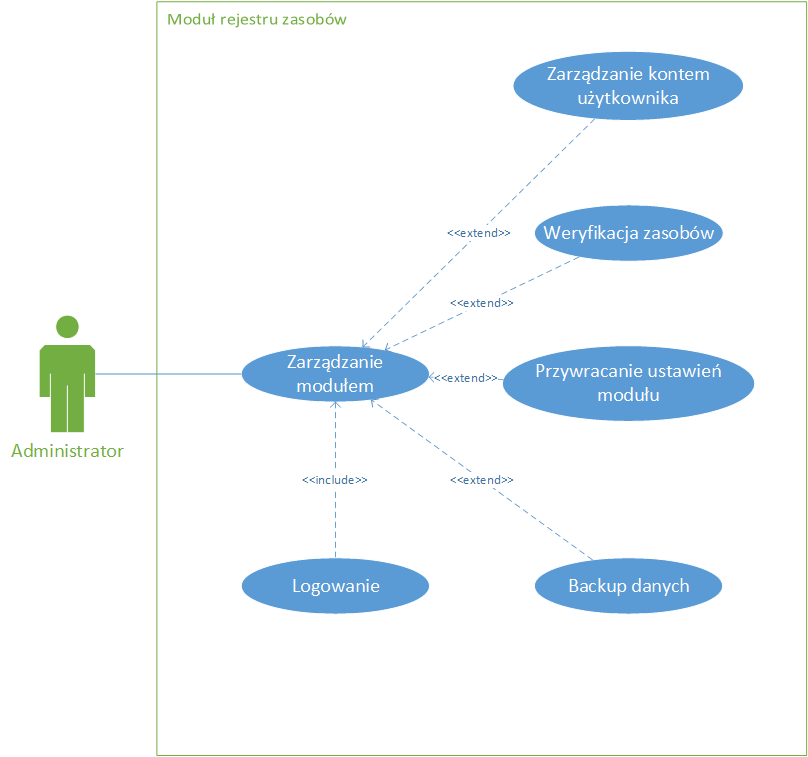
\includegraphics[scale=1]{Zarzadzanie_modulem.png}
\end{figure}

\paragraph{Warunki wstępne:} Administrator musi być zalogowany.
\paragraph{Warunki końcowe:} Administrator musi zatwierdzić zmiany w ustawieniach modułu.

\section{Zarządzanie kontem użytkownika}
\paragraph{Opis przypadku użycia:} Administrator ma możliwość zarządzania kontem danego użytkownika modułu.
\paragraph{Priorytet:} 8
\paragraph{Aktorzy:} Administrator
\paragraph{Podstawowy przebieg:}
\begin{enumerate}
\item Administrator ma możliwość wybrania użytkownika.
\item Administrator ma możliwosć zatwierdzenia konta.
\item Administrator ma możliwosć edycji praw konta użytkownika.
\item Administrator ma możliwosć usunięcia konta użytkownika z modułu.
\end{enumerate}

\begin{figure}[H]
Diagram przypadku użycia:

\centering
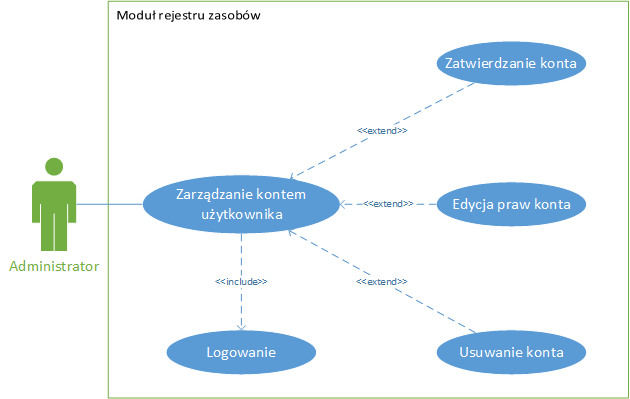
\includegraphics[scale=1]{Zarzadzanie_kontem.png}
\end{figure}

\paragraph{Warunki wstępne:} Administrator musi być zalogowany.
\paragraph{Warunki końcowe:} Zmiany dotyczące ustawień konta danego użytkownika zostają zarejestrowane w systemie.

\section{Weryfikacja zasobów}

\paragraph{Opis przypadku użycia:} Administrator może weryfikować zasoby znajdujące się w systemie.
\paragraph{Priorytet:} 8
\paragraph{Aktorzy:} Administrator
\paragraph{Podstawowy przebieg:}
\begin{enumerate}
\item Administrator może weryfikować dostępne zasoby (sprawdzać stan i parametry).
\item Administrator może sprawdzić historię wybranego zasobu.
\end{enumerate}

\begin{figure}[H]
Diagram przypadku użycia:

\centering
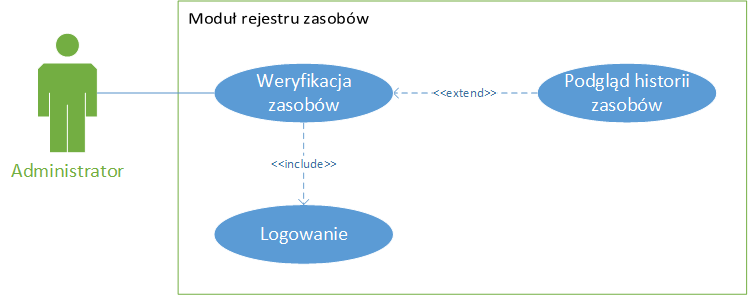
\includegraphics[scale=1]{weryfikacja_zasobow.png}
\end{figure}

\paragraph{Warunki wstępne:} Administrator musi być zalogowany.
\paragraph{Warunki końcowe:} ---

\section{Raportowanie}
\paragraph{Opis przypadku użycia:} 
Użytkownik techniczny/Administrator ma możliwość wygenerowania raportu dotyczącego zasobów w systemie do pliku pdf.
\paragraph{Priorytet:} 6
\paragraph{Aktorzy:} Użytkownik techniczny, Administrator
\paragraph{Podstawowy przebieg:}
\begin{enumerate}
\item Użytkownik techniczny/Administrator wybiera kryteria podglądu zasobów.
\item Użytkownik techniczny/Administrator generuje raport dotyczący wybranych zasobów. 
\end{enumerate}

\begin{figure}[H]
Diagram przypadku użycia:

\centering
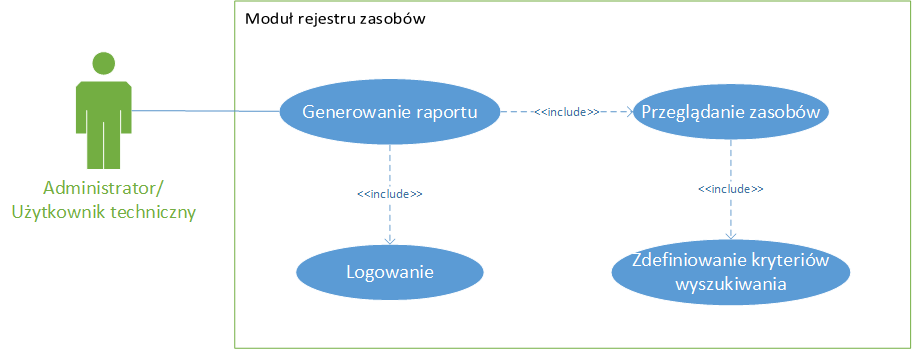
\includegraphics[scale=0.8]{techniczny_i_admin_raporty.png}
\end{figure}

\paragraph{Warunki wstępne:} Administrator musi być zalogowany.
\paragraph{Warunki końcowe:} ---

\section{Definiowanie typów zasobów}
\paragraph{Opis przypadku użycia:} 
Administrator ma możliwość zdefiniowania nowego typu zasobu w systemie.
\paragraph{Priorytet:} 10
\paragraph{Aktorzy:} Użytkownik techniczny, Administrator
\paragraph{Podstawowy przebieg:}
\begin{enumerate}
\item Administrator definiuje nowy typ zasobu i opisujące go parametry.
\item Administrator zatwierdza i wprowadza do systemu nowy typ zasobu. 
\end{enumerate}

\begin{figure}[H]
Diagram przypadku użycia:

\centering
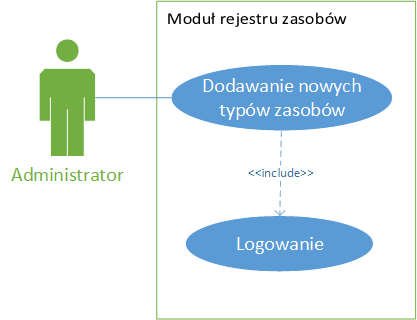
\includegraphics[scale=0.8]{admin_dodawanie_typow.png}
\end{figure}

\paragraph{Warunki wstępne:} Administrator musi być zalogowany.
\paragraph{Warunki końcowe:} Nowy typ zasobu zostaje dodany do systemu.

\chapter{Diagramy klas i diagramy sekwencji}
\counterwithin{subsection}{section}
\renewcommand{\thesection}{\colorbox{gray}{\textcolor{white}{CSD%
\arabic{section}}}}

\section{Logowanie użytkownika}
\begin{figure}[H]
\centering
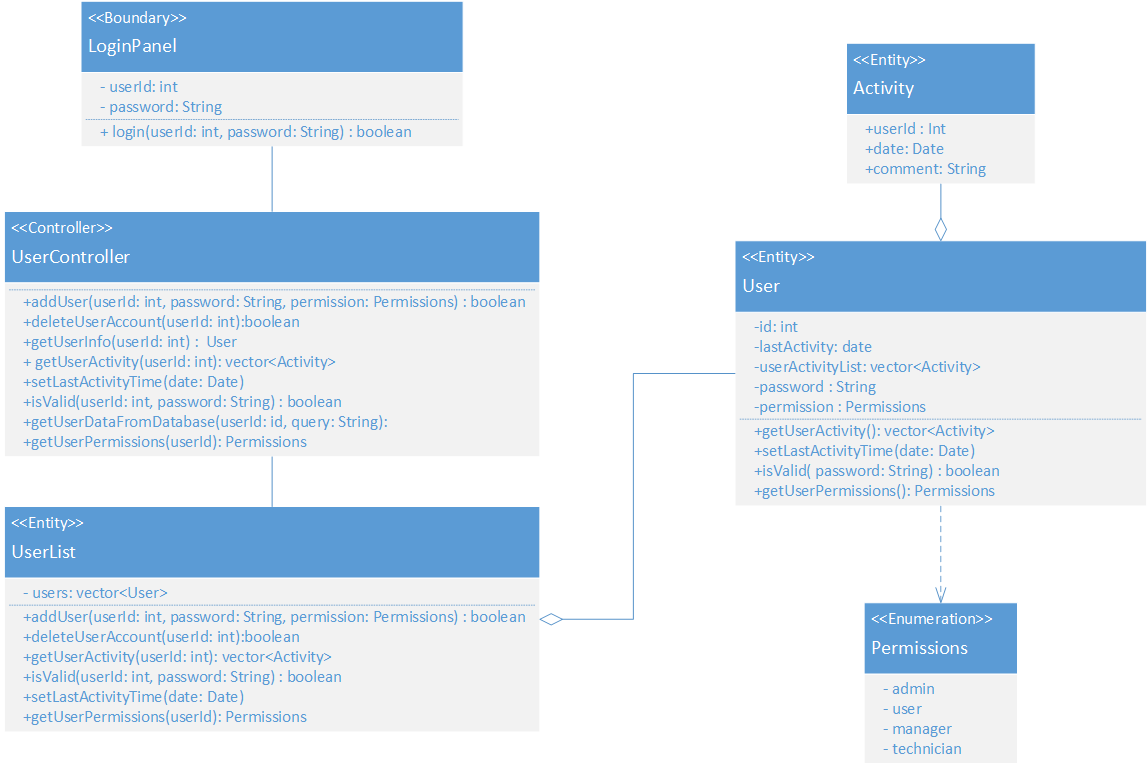
\includegraphics[scale=0.5]{logowanie_class.png}
\end{figure}
\begin{figure}[H]
\centering
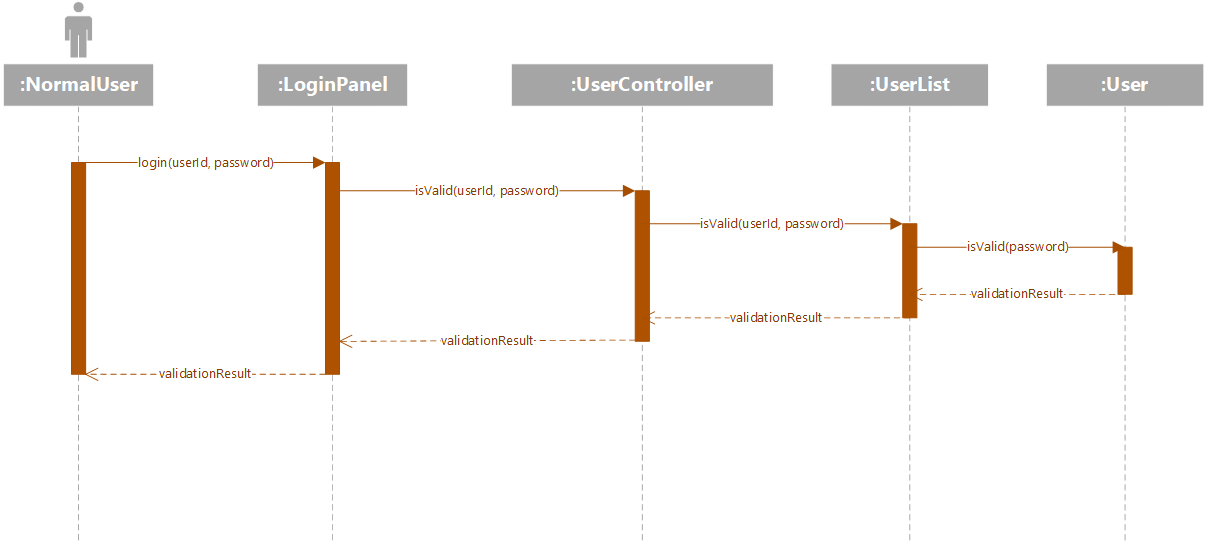
\includegraphics[scale=0.5]{logowanie_sequence.png}
\end{figure}

\section{Rejestracja użytkownika}
\begin{figure}[H]
\centering
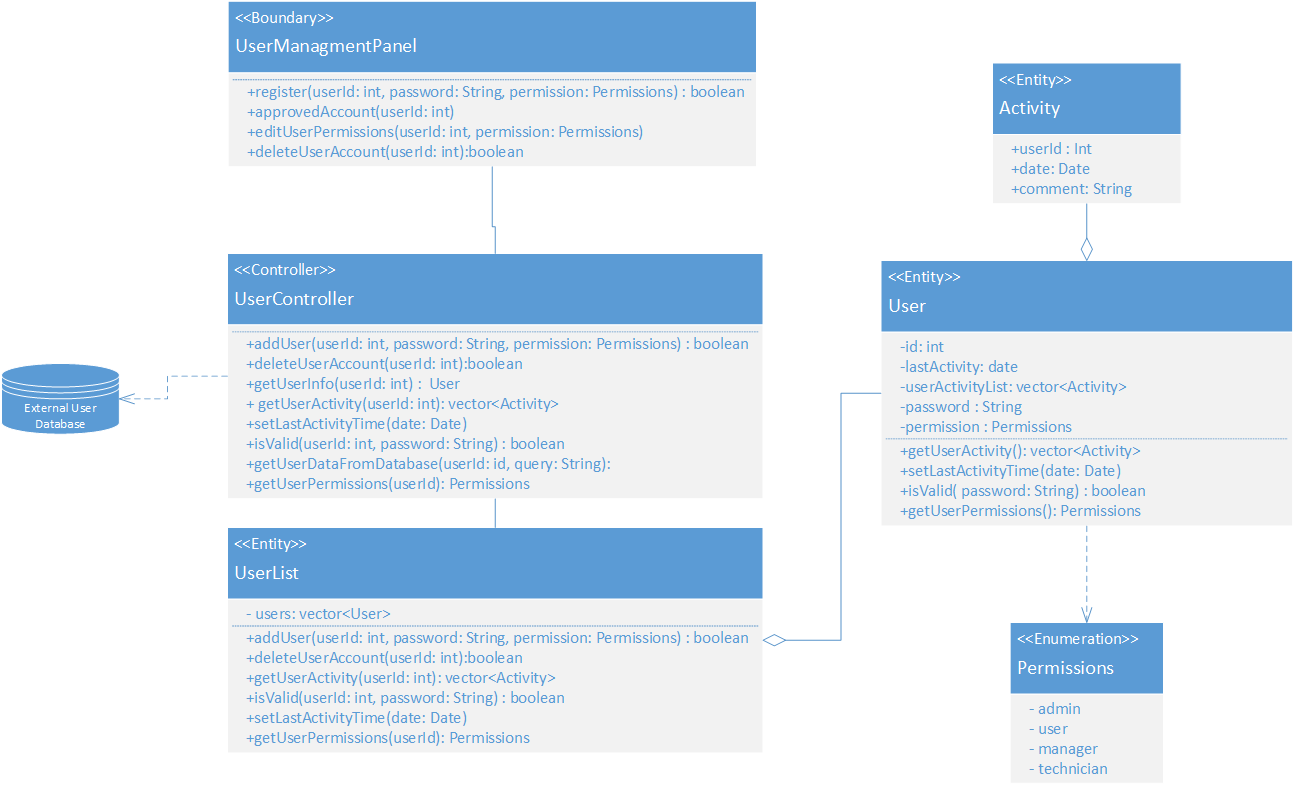
\includegraphics[scale=0.5]{rejestracja_class.png}
\end{figure}
\begin{figure}[H]
\centering
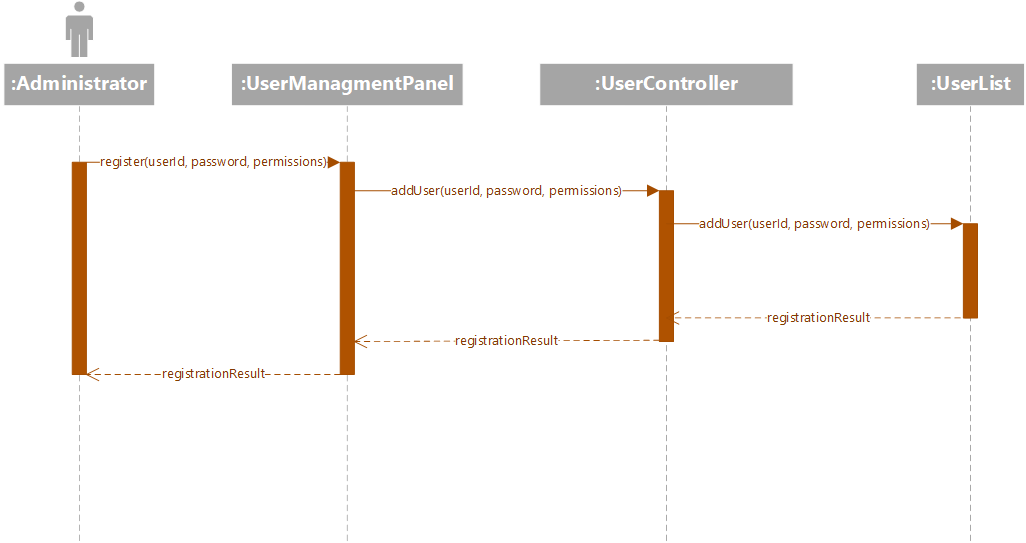
\includegraphics[scale=0.5]{rejestracja_sequence.png}
\end{figure}

\section{Zgłoszenie o przyznanie nowego zasobu}
\begin{figure}[H]
\centering
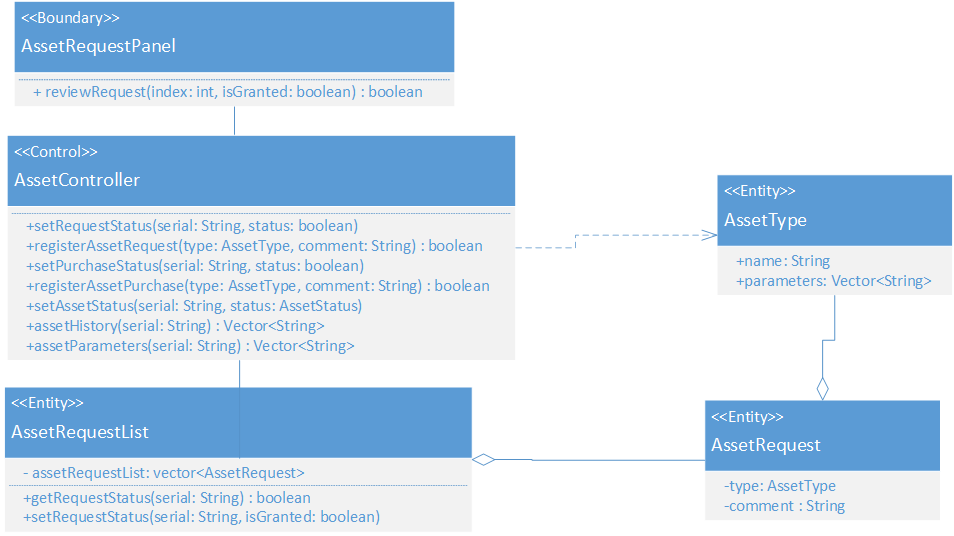
\includegraphics[scale=0.5]{zgloszenie_zasob_class.png}
\end{figure}
\begin{figure}[H]
\centering
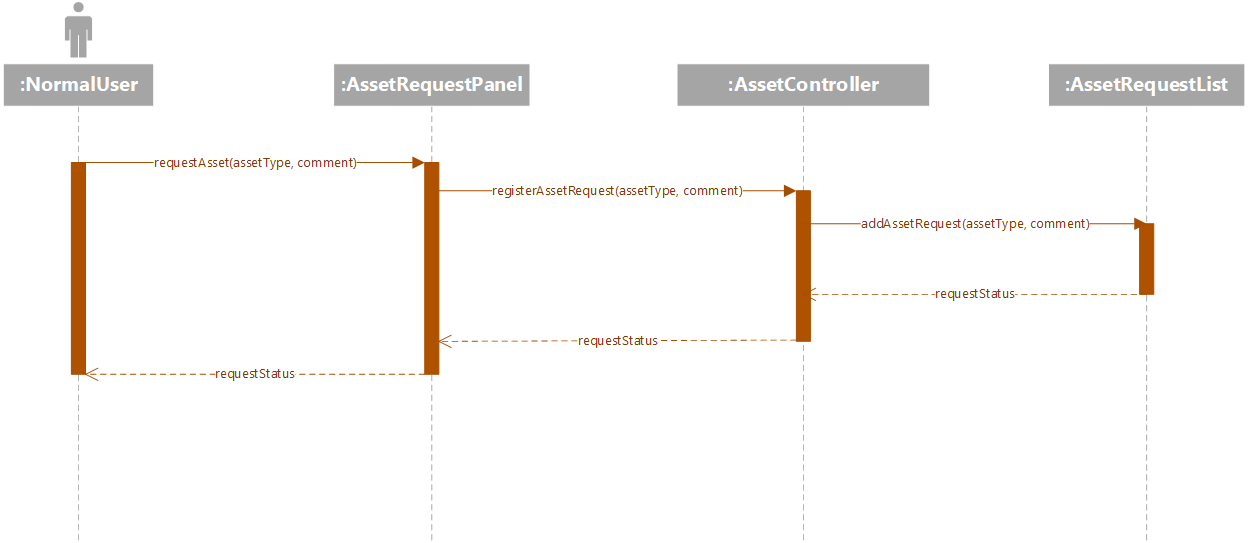
\includegraphics[scale=0.5]{zgloszenie_zasob_sequence.png}
\end{figure}

\section{Zatwierdzenie prośby o przyznanie nowego zasobu}
\begin{figure}[H]
\centering
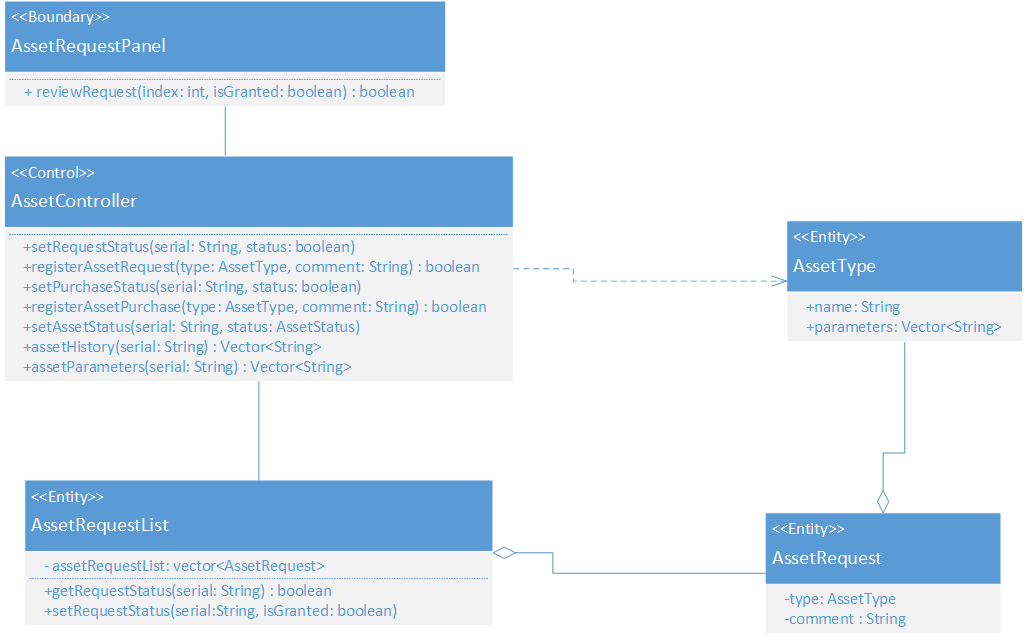
\includegraphics[scale=0.5]{zatwierdzenie_zasob_class.png}
\end{figure}
\begin{figure}[H]
\centering
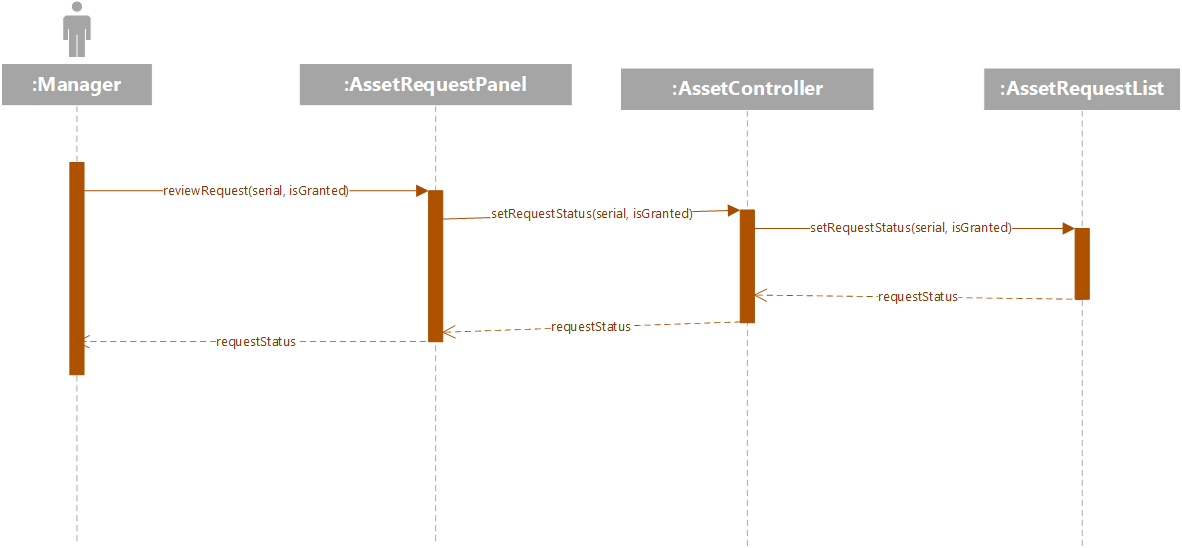
\includegraphics[scale=0.5]{zatwierdzenie_zasob_sequence.png}
\end{figure}

\section{Wydanie zasobu}
\begin{figure}[H]
\centering
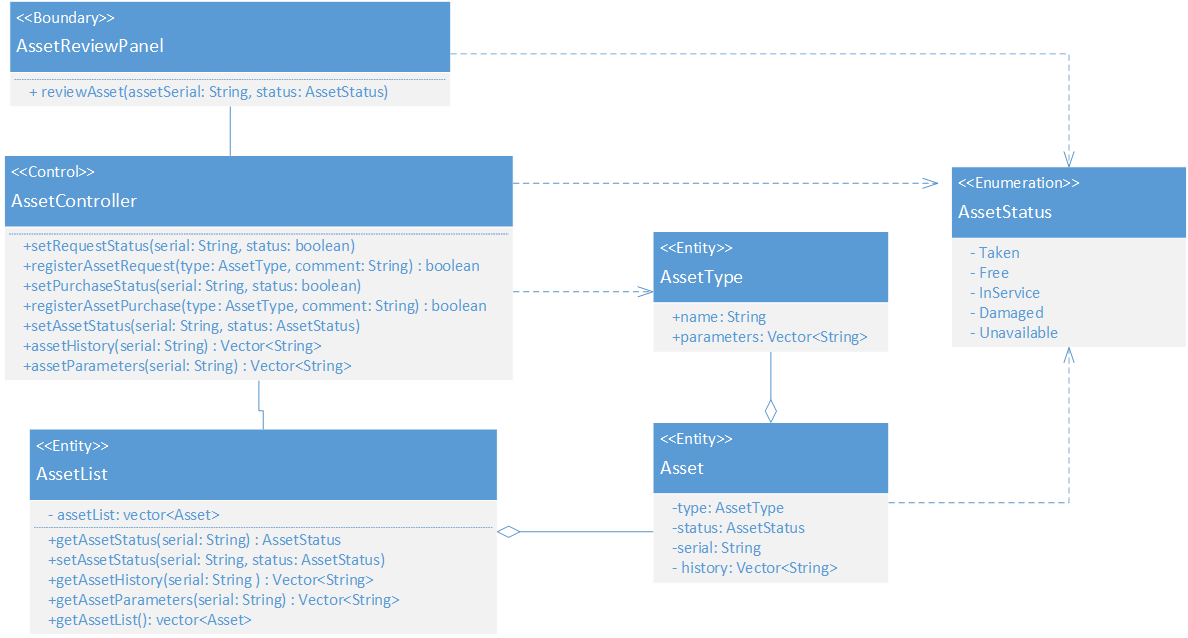
\includegraphics[scale=0.5]{techniczny_wydanie_zasobu_class.png}
\end{figure}
\begin{figure}[H]
\centering
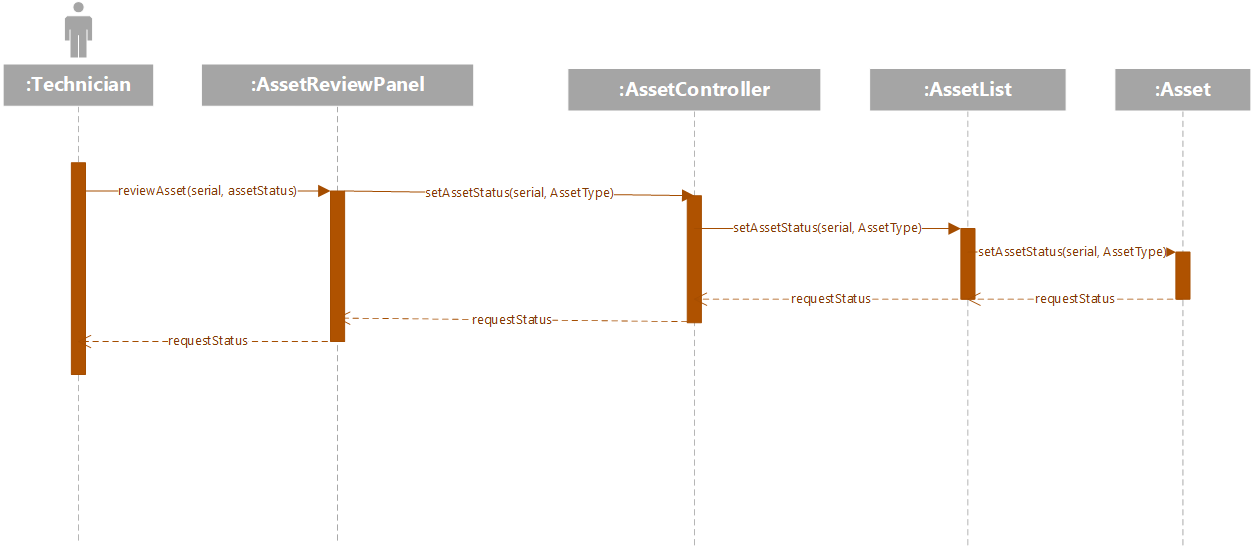
\includegraphics[scale=0.5]{techniczny_wydanie_zasobu_sequence.png}
\end{figure}

\section{Zgłoszenie zasobu do serwisu}
\begin{figure}[H]
\centering
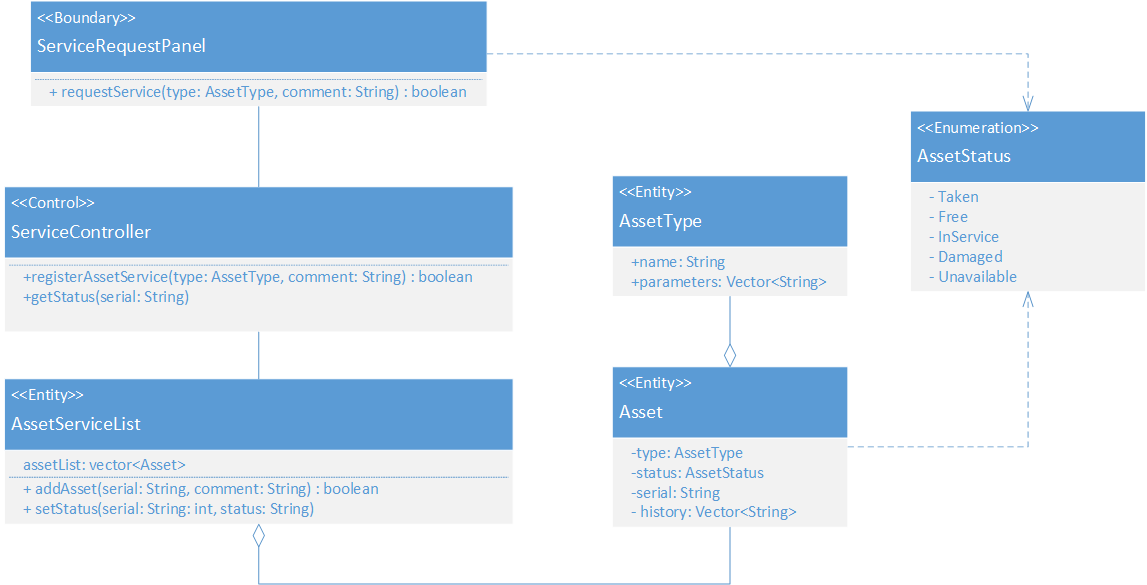
\includegraphics[scale=0.5]{zgloszenie_serwis_class.png}
\end{figure}
\begin{figure}[H]
\centering
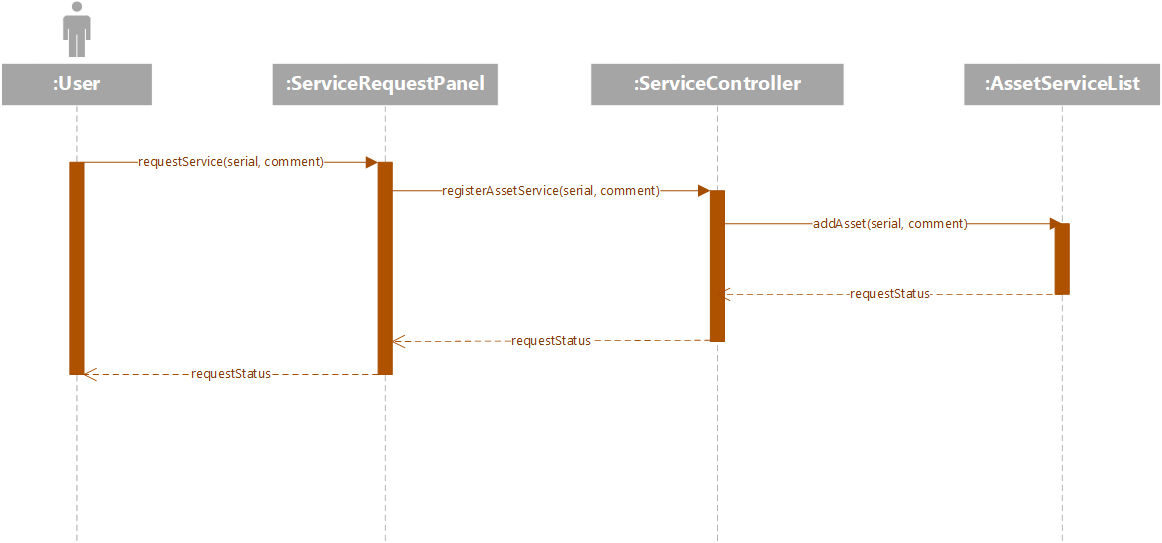
\includegraphics[scale=0.5]{zgloszenie_serwis_sequence.png}
\end{figure}

\section{Przyjęcie zgłoszenia serwisowego}
\begin{figure}[H]
\centering
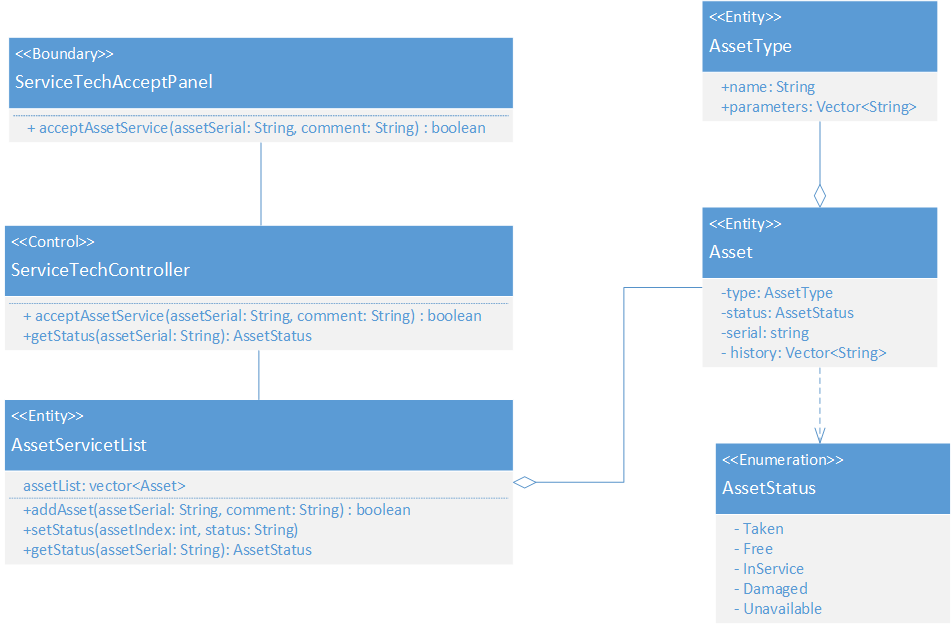
\includegraphics[scale=0.5]{przyjecie_zgloszenia_serwis_class.png}
\end{figure}
\begin{figure}[H]
\centering
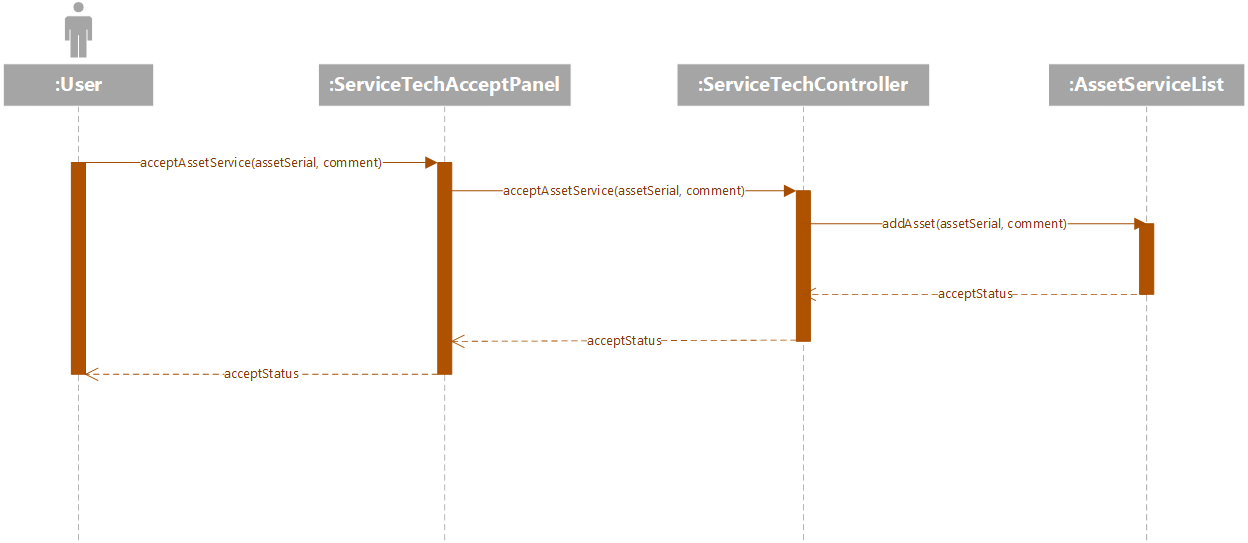
\includegraphics[scale=0.5]{przyjecie_zgloszenia_serwis_sequence.png}
\end{figure}

\section{Wylogowanie}
\begin{figure}[H]
\centering
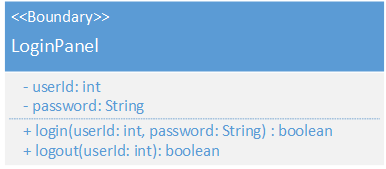
\includegraphics[scale=0.5]{wylogowanie_class.png}
\end{figure}
\begin{figure}[H]
\centering
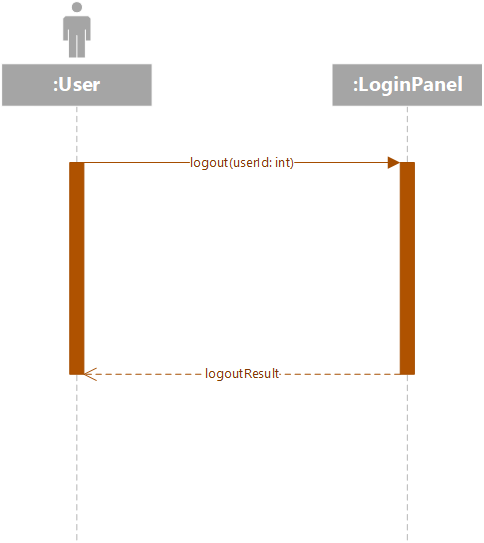
\includegraphics[scale=0.5]{wylogowanie_sequence.png}
\end{figure}

\section{Zgłoszenie o kupno zasobu}
\begin{figure}[H]
\centering
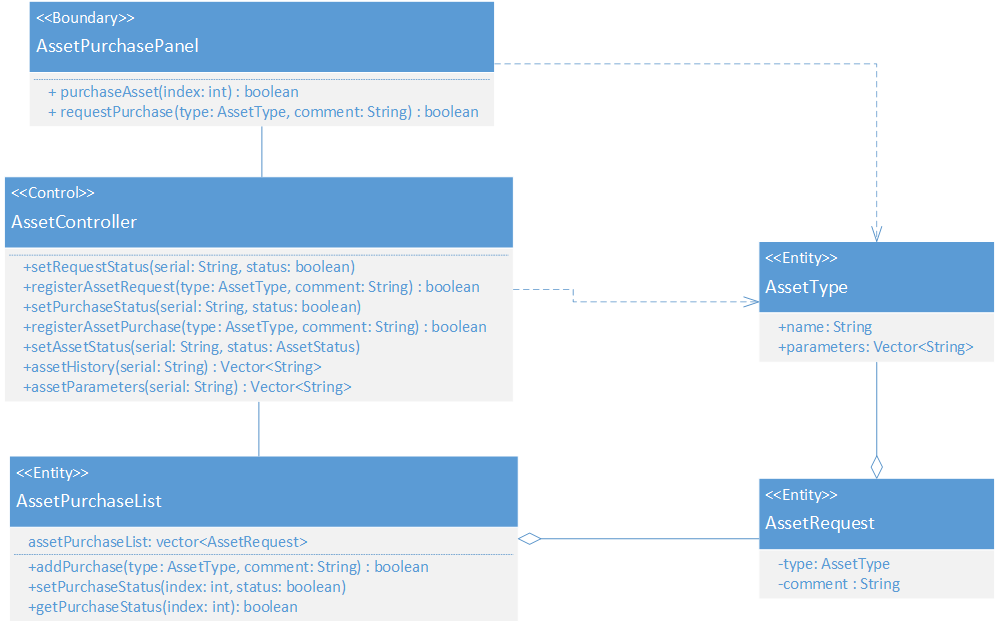
\includegraphics[scale=0.5]{zgloszenie_kupno_zasob_class.png}
\end{figure}
\begin{figure}[H]
\centering
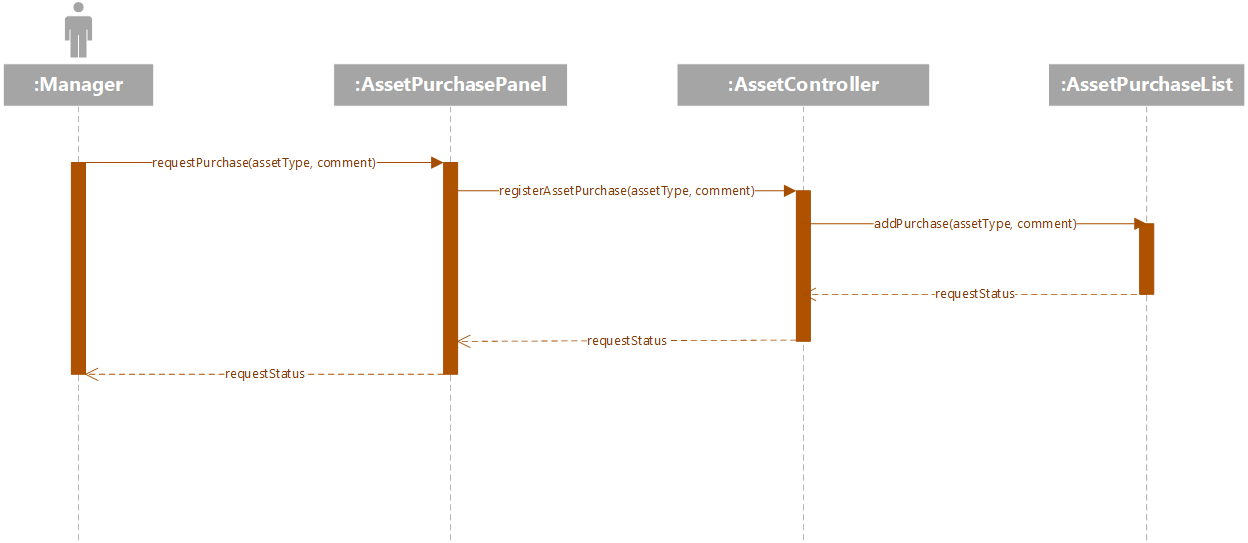
\includegraphics[scale=0.5]{zgloszenie_kupno_zasob_sequence.png}
\end{figure}

\section{Kupno zasobu}
\begin{figure}[H]
\centering
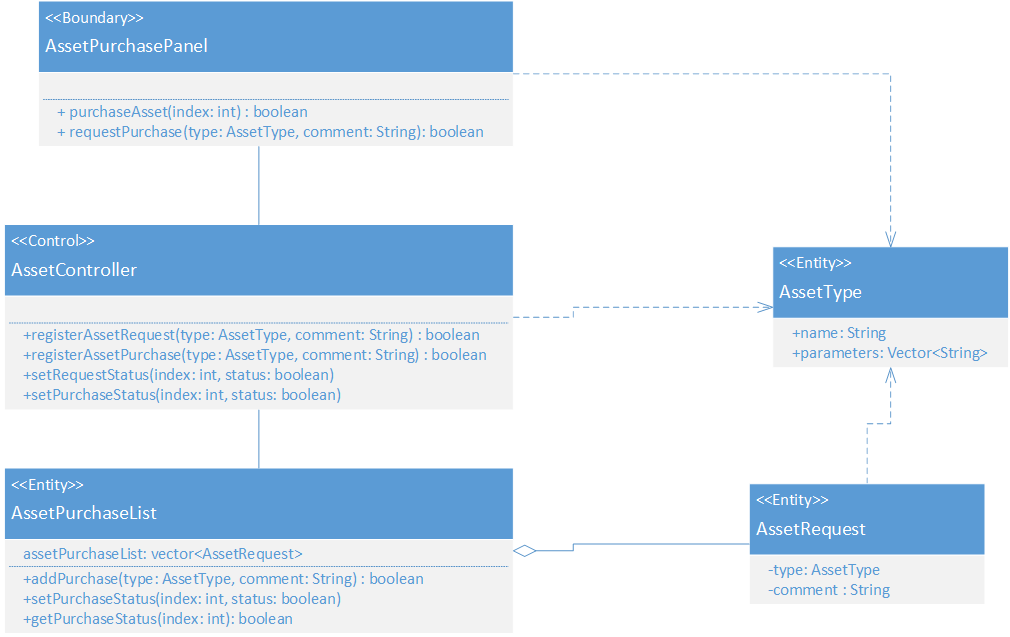
\includegraphics[scale=0.5]{kupno_zasob_class.png}
\end{figure}
\begin{figure}[H]
\centering
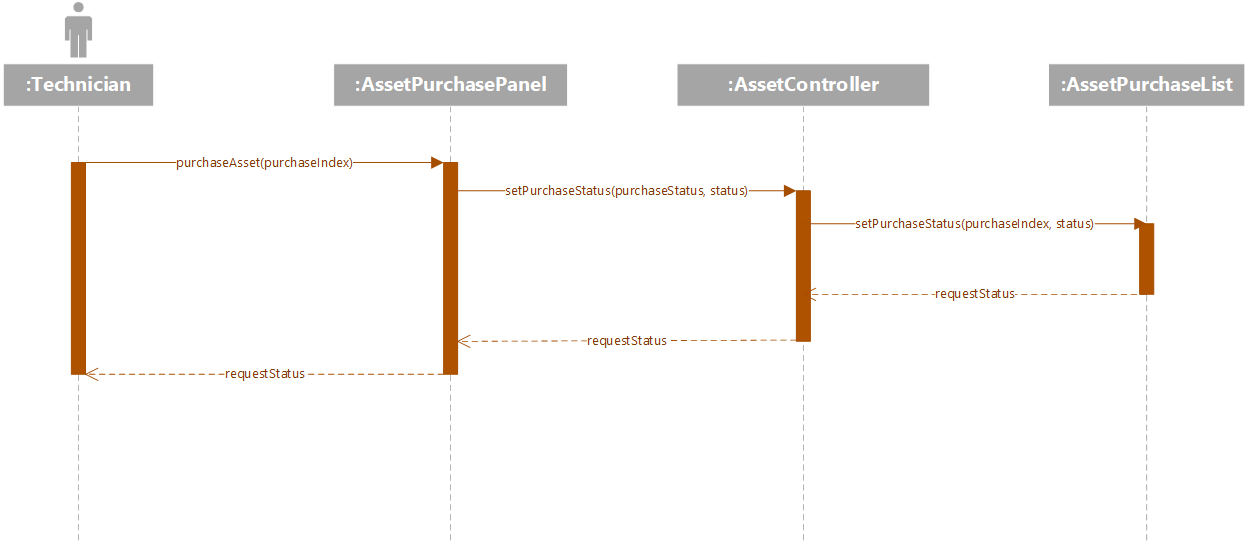
\includegraphics[scale=0.5]{kupno_zasob_sequence.png}
\end{figure}

\section{Podgląd historii użytkowników}
\begin{figure}[H]
\centering
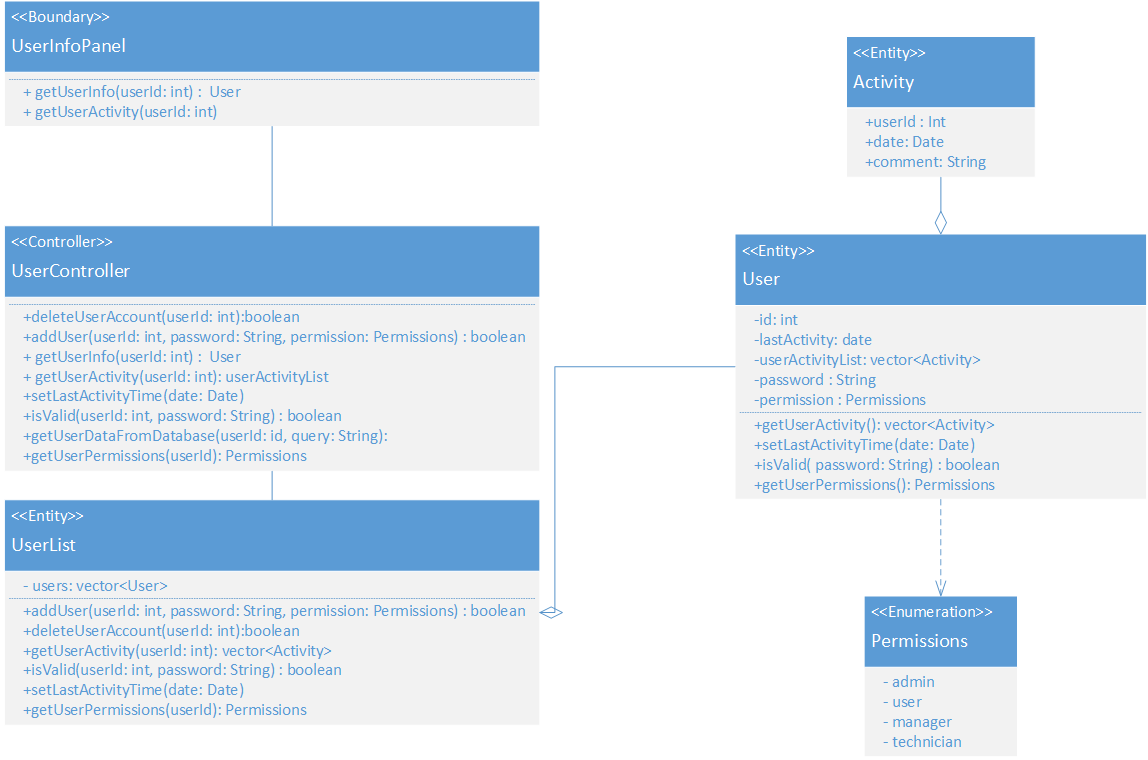
\includegraphics[scale=0.5]{podglad_historii_class.png}
\end{figure}
\begin{figure}[H]
\centering
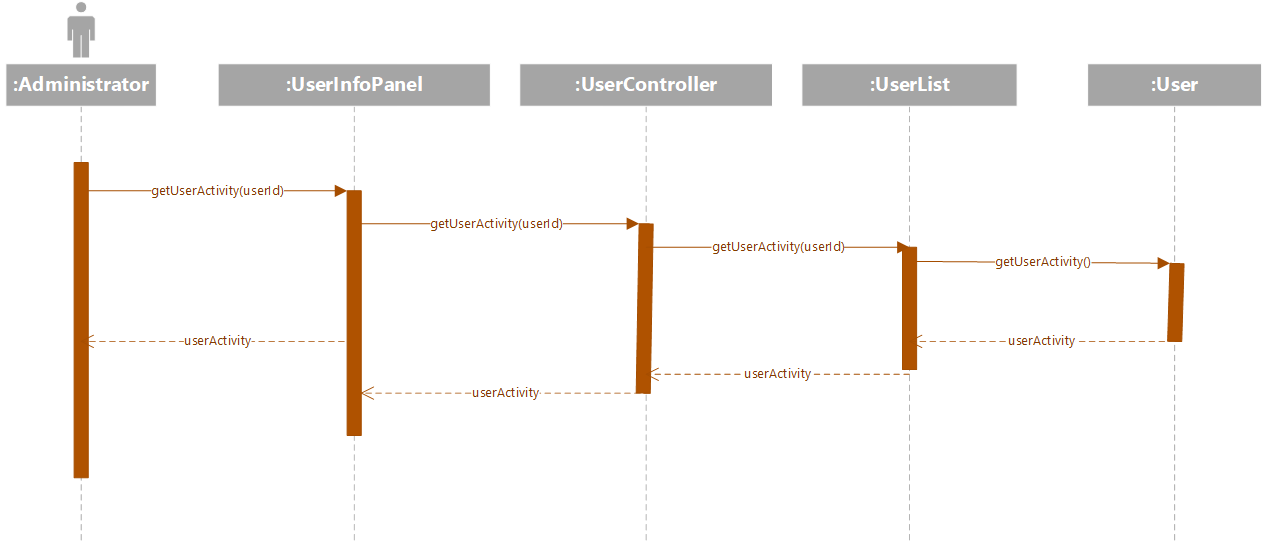
\includegraphics[scale=0.5]{podglad_historii_sequence.png}
\end{figure}

\section{Zarządzanie modułem}
\begin{figure}[H]
\centering
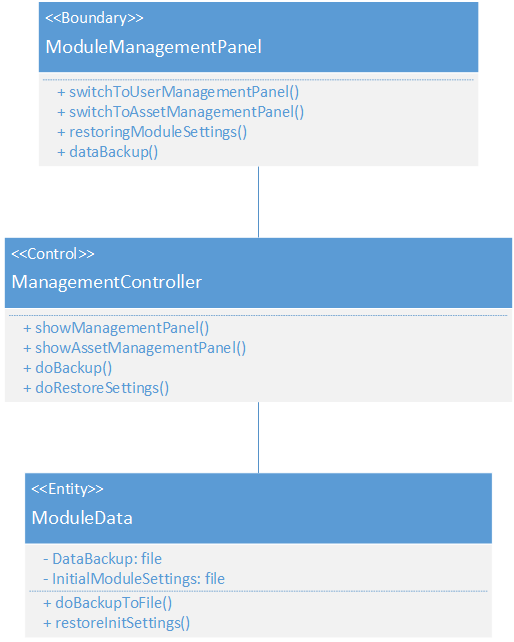
\includegraphics[scale=0.5]{zarzadzanie_modulem_class.png}
\end{figure}
\begin{figure}[H]
\centering
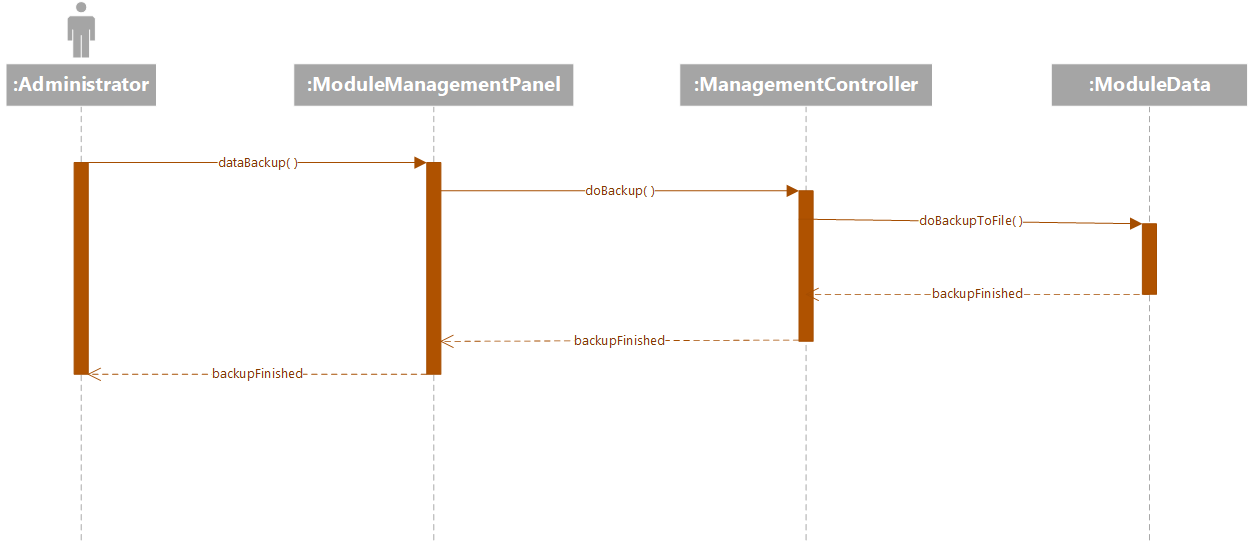
\includegraphics[scale=0.5]{backup.png}
\end{figure}
\begin{figure}[H]
\centering
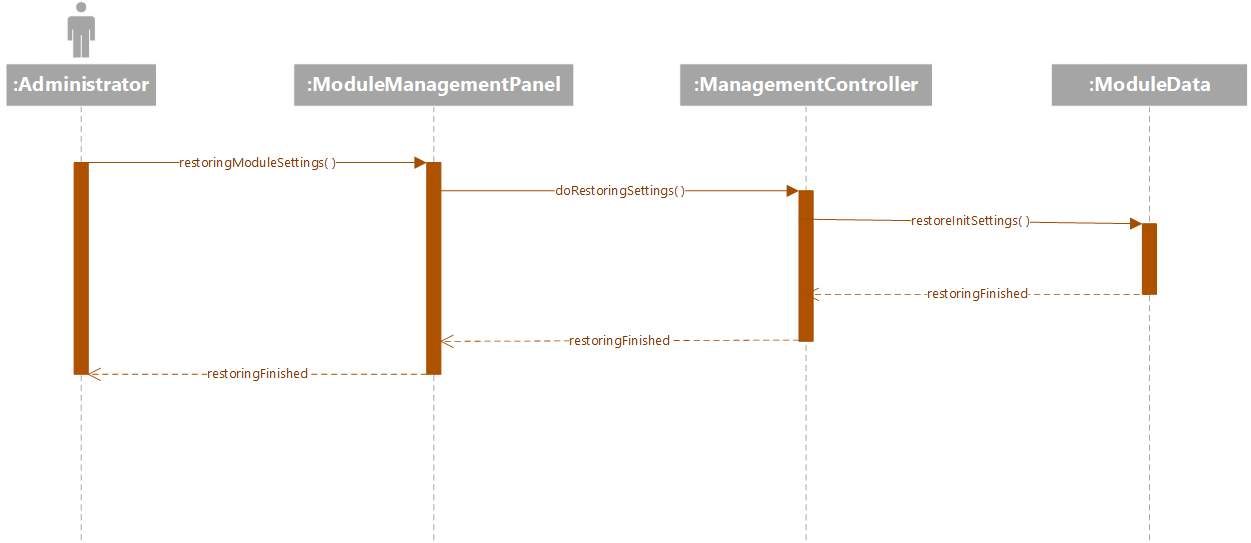
\includegraphics[scale=0.5]{restoring.png}
\end{figure}

\section{Zarządzanie kontem użytkownika}
\begin{figure}[H]
\centering
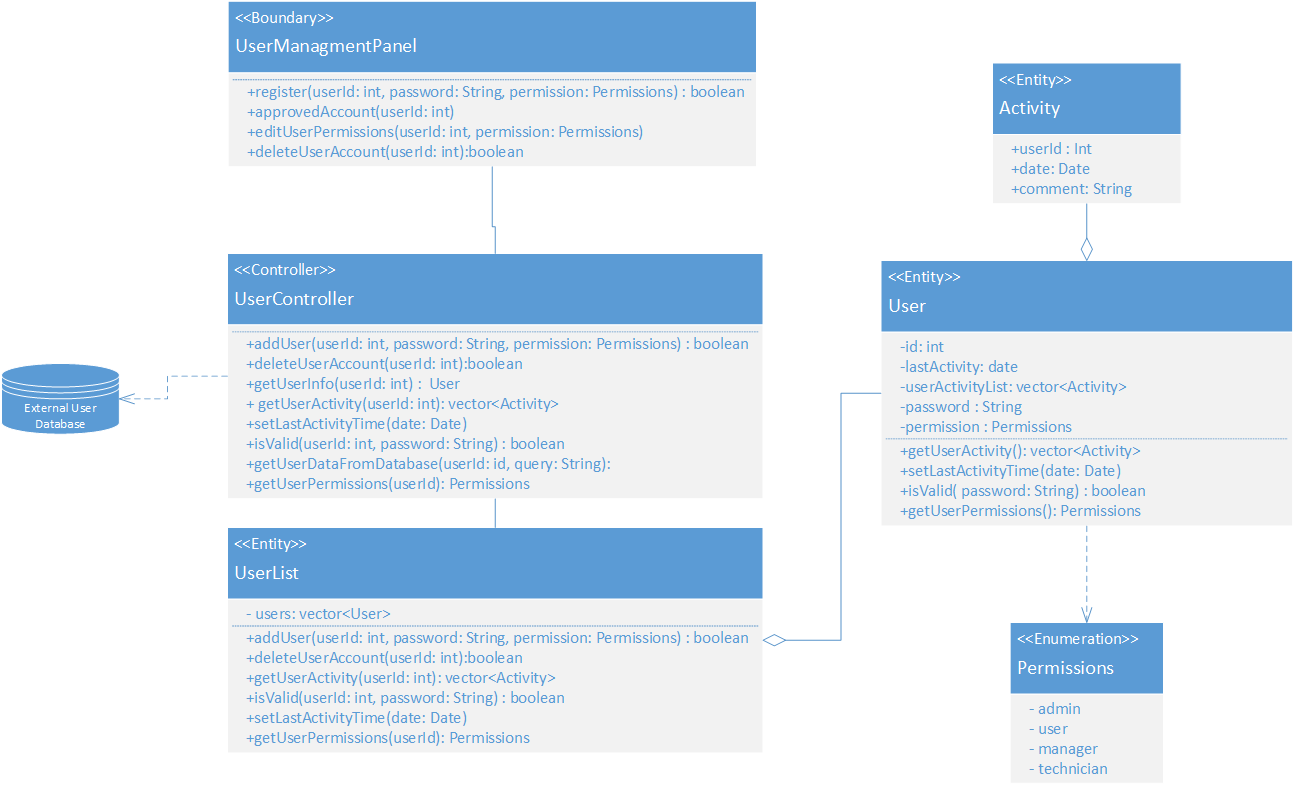
\includegraphics[scale=0.5]{zarzadzanie_uzytkownikami_class.png}
\end{figure}
\begin{figure}[H]
\centering
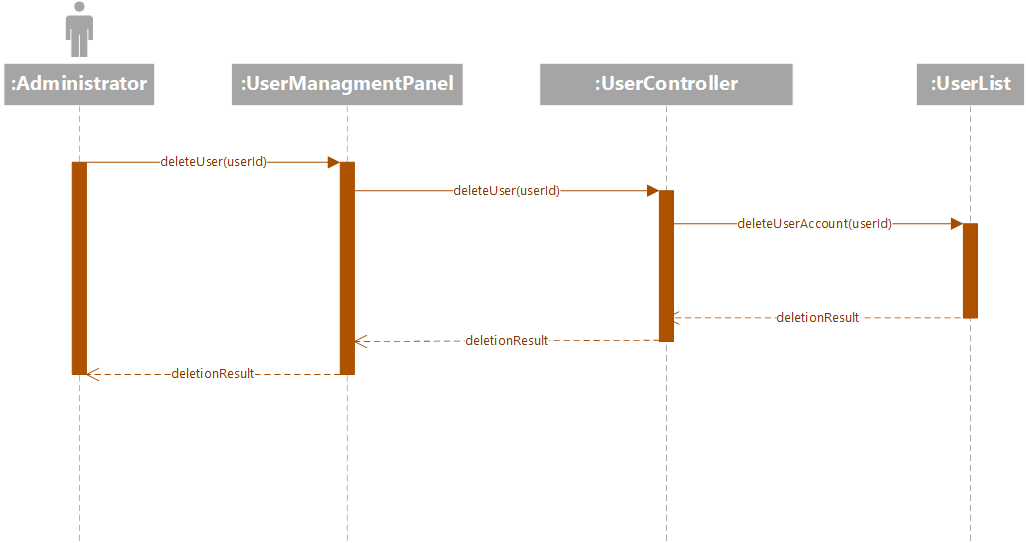
\includegraphics[scale=0.5]{zarzadzanie_uzytkownikami_sequence.png}
\end{figure}

\section{Weryfikacja zasobów}
\begin{figure}[H]
\centering
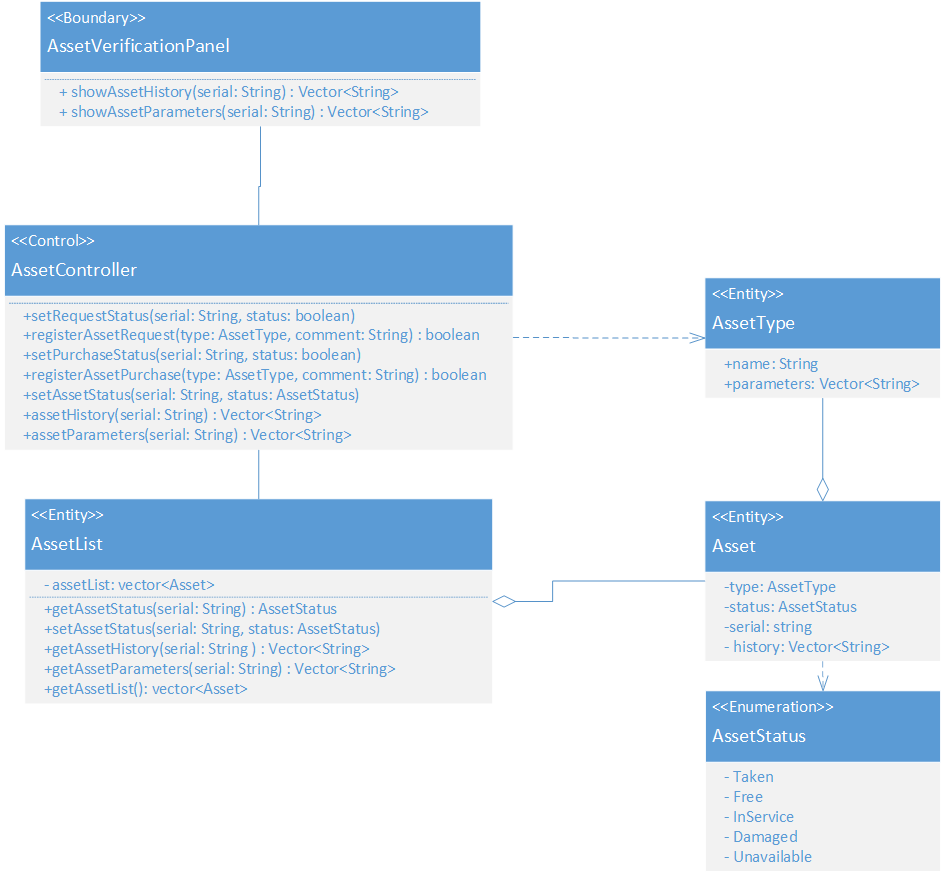
\includegraphics[scale=0.5]{weryfikacja.png}
\end{figure}
\begin{figure}[H]
\centering
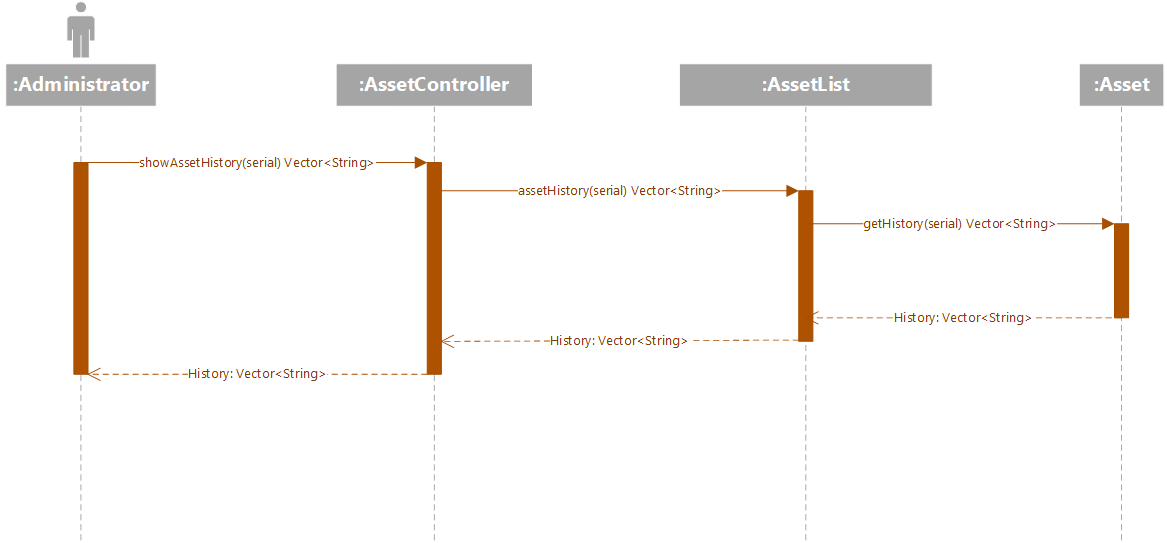
\includegraphics[scale=0.5]{weryfikacja_sequence.png}
\end{figure}

\section{Raportowanie}
\begin{figure}[H]
\centering
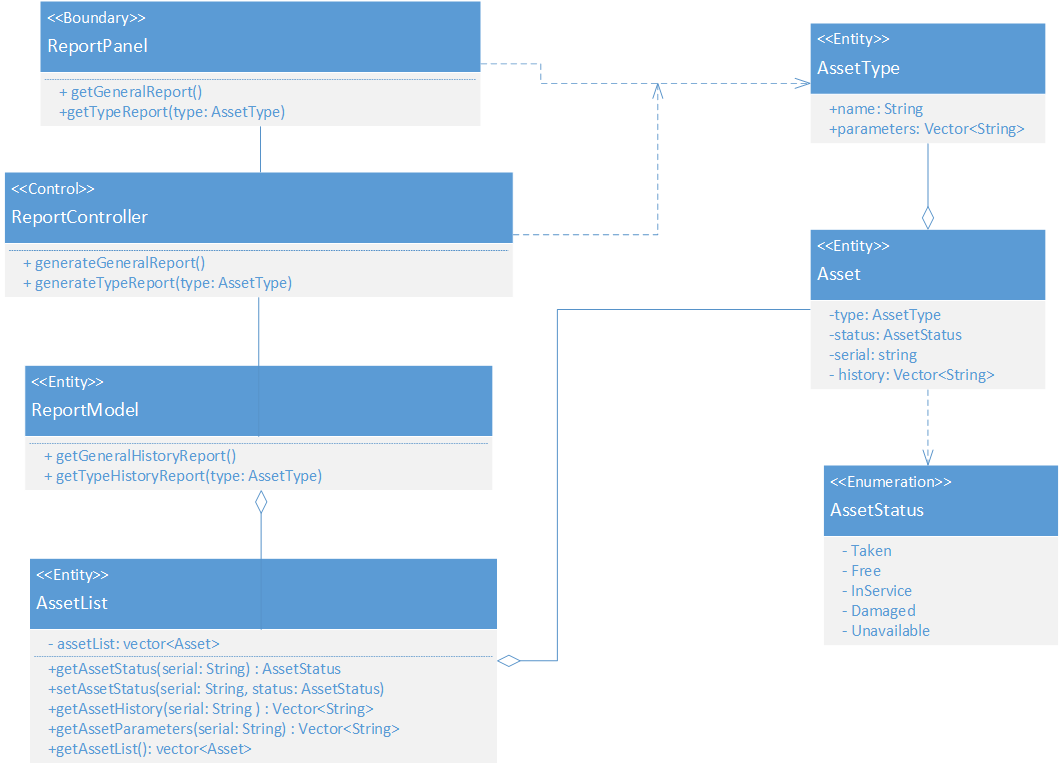
\includegraphics[scale=0.5]{raportowanie_class.png}
\end{figure}
\begin{figure}[H]
\centering
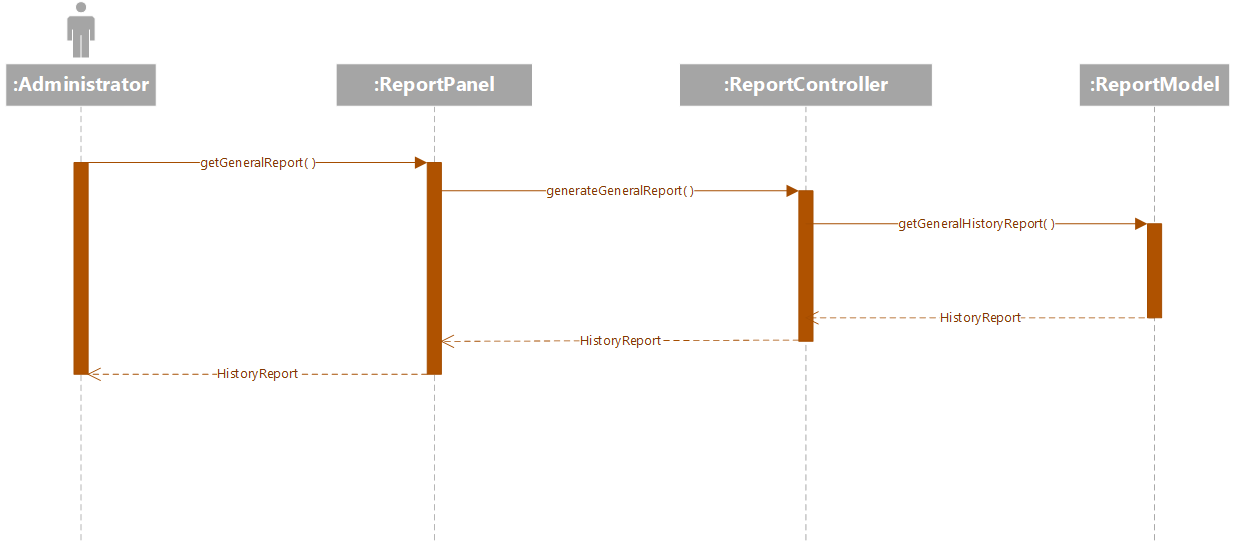
\includegraphics[scale=0.5]{raportowanie_sequence.png}
\end{figure}
\section{Definiowanie typów zasobów}
\begin{figure}[H]
\centering
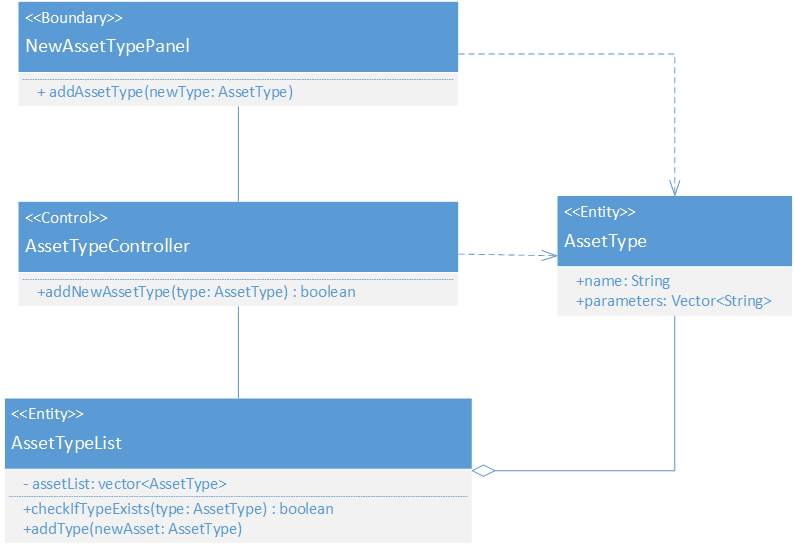
\includegraphics[scale=0.5]{nowy_typ_zasob_class.png}
\end{figure}
\begin{figure}[H]
\centering
\includegraphics[scale=0.5]{nowy_typ_zasob_sequence.png}
\end{figure}

\chapter{Diagram komponentów}

\begin{figure}[H]
\centering
\includegraphics[scale=0.5]{components_diagram.png}
\end{figure}

\chapter{Model bazy danych}

\begin{figure}[H]
\centering
\includegraphics[scale=0.5]{database.png}
\end{figure}

\pagebreak

\chapter{Interfejs użytkownika}
Poniżej zamieszczono przykładowe elementy interfejsu użytkownika: 

\begin{figure}[H]
\centering
\includegraphics[scale=0.5]{login_panel.png}
\captionof{figure}{Panel logowania}
\end{figure}

\begin{figure}[H]
\centering
\includegraphics[scale=0.5]{logout_panel.png}
\captionof{figure}{Okno wylogowania}
\end{figure}

\begin{figure}[H]
\centering
\includegraphics[scale=0.8]{register_user_panel.png}
\captionof{figure}{Panel rejestrowania nowego użytkownika}
\end{figure}

\begin{figure}[H]
\centering
\includegraphics[scale=0.45]{admin_panel.png}
\captionof{figure}{Panel administratora- karta zasobów}
\end{figure}

\begin{figure}[H]
\centering
\includegraphics[scale=0.45]{admin_panel_user_management.png}
\captionof{figure}{Panel administratora- karta zarządzania użytkownikami}
\end{figure}

\begin{figure}[H]
\centering
\includegraphics[scale=0.45]{admin_panel_reports.png}
\captionof{figure}{Panel administratora- karta raportów}
\end{figure}

\end{document}



